% -*- coding: utf-8 -*-
%-------------------------designed by zcf--------------
\documentclass[UTF8,a4paper,10pt]{ctexart}
\usepackage[left=3.17cm, right=3.17cm, top=2.74cm, bottom=2.74cm]{geometry}
\usepackage{amsmath}
\usepackage{graphicx}
\usepackage{wrapfig}
% \usepackage{subcaption}  % 子图支持
\usepackage{float}
\usepackage{cite}
\usepackage{caption}
\usepackage{siunitx} % 单位支持宏包
\usepackage{enumerate}
\usepackage{booktabs} %表格
\usepackage{multirow}
\usepackage{tabularx} % 在导言区添加
\usepackage{ctex}
% ctex 会自动选择合适的系统字体，无需手动指定
\newcommand{\tabincell}[2]{\begin{tabular}{@{}#1@{}}#2\end{tabular}}  %表格强制换行
%-------------------------字体设置--------------
% \usepackage{times}
\newcommand{\yihao}{\fontsize{26pt}{36pt}\selectfont}           % 一号, 1.4 倍行距
\newcommand{\erhao}{\fontsize{22pt}{28pt}\selectfont}          % 二号, 1.25倍行距
\newcommand{\xiaoer}{\fontsize{18pt}{18pt}\selectfont}          % 小二, 单倍行距
\newcommand{\sanhao}{\fontsize{16pt}{24pt}\selectfont}  %三号字
\newcommand{\xiaosan}{\fontsize{15pt}{22pt}\selectfont}        % 小三, 1.5倍行距
\newcommand{\sihao}{\fontsize{14pt}{21pt}\selectfont}            % 四号, 1.5 倍行距
\newcommand{\banxiaosi}{\fontsize{13pt}{19.5pt}\selectfont}    % 半小四, 1.5倍行距
\newcommand{\xiaosi}{\fontsize{12pt}{18pt}\selectfont}            % 小四, 1.5倍行距
\newcommand{\dawuhao}{\fontsize{11pt}{11pt}\selectfont}       % 大五号, 单倍行距
\newcommand{\wuhao}{\fontsize{10.5pt}{15.75pt}\selectfont}    % 五号, 单倍行距

\usepackage{amsmath}
\usepackage{xeCJK}
%-------------------------章节名----------------
\usepackage{ctexcap}
\CTEXsetup[name={,、},number={ \chinese{section}}]{section}
\CTEXsetup[name={（,）},number={\chinese{subsection}}]{subsection}
\CTEXsetup[name={,.},number={\arabic{subsubsection}}]{subsubsection}
%-------------------------页眉页脚--------------
\usepackage{fancyhdr}
\pagestyle{fancy}
\lhead{\kaishu \leftmark}
% \chead{}
\rhead{\kaishu 软件工程实验报告}%加粗\bfseries
\lfoot{}
\cfoot{\thepage}
\rfoot{}
\renewcommand{\headrulewidth}{0.1pt}
\renewcommand{\footrulewidth}{0pt}%去掉横线
\newcommand{\HRule}{\rule{\linewidth}{0.5mm}}%标题横线
\newcommand{\HRulegrossa}{\rule{\linewidth}{1.2mm}}
%-----------------------伪代码------------------
\usepackage{algorithm}
\usepackage{algorithmicx}
\usepackage{algpseudocode}
\floatname{algorithm}{Algorithm}
\renewcommand{\algorithmicrequire}{\textbf{Input:}}
\renewcommand{\algorithmicensure}{\textbf{Output:}}
\usepackage{lipsum}
\makeatletter
\newenvironment{breakablealgorithm}
  {% \begin{breakablealgorithm}
  \begin{center}
     \refstepcounter{algorithm}% New algorithm
     \hrule height.8pt depth0pt \kern2pt% \@fs@pre for \@fs@ruled
     \renewcommand{\caption}[2][\relax]{% Make a new \caption
      {\raggedright\textbf{\ALG@name~\thealgorithm} ##2\par}%
      \ifx\relax##1\relax % #1 is \relax
         \addcontentsline{loa}{algorithm}{\protect\numberline{\thealgorithm}##2}%
      \else % #1 is not \relax
         \addcontentsline{loa}{algorithm}{\protect\numberline{\thealgorithm}##1}%
      \fi
      \kern2pt\hrule\kern2pt
     }
  }{% \end{breakablealgorithm}
     \kern2pt\hrule\relax% \@fs@post for \@fs@ruled
  \end{center}
  }
\makeatother
%------------------------代码-------------------
\usepackage{xcolor}
\usepackage{listings}
\usepackage{minted}
\lstset{
  language=C,                     % 指定语言
  breaklines=true,                % 自动换行
  basicstyle=\small\ttfamily,     % 代码字体
  escapeinside=``,
  keywordstyle=\color{blue!70}\bfseries,
  commentstyle=\itshape\color{green!50!black}, % 注释颜色
  stringstyle=\ttfamily\color{orange},         % 字符串颜色
  extendedchars=false,
  linewidth=\textwidth,
  numbers=left,
  numberstyle=\tiny\color{blue!50},
  frame=trbl%,
  rulesepcolor=\color{red!20!green!20!blue!20}
}
%------------超链接----------
\usepackage[colorlinks,linkcolor=black,anchorcolor=blue]{hyperref}
%------------------------TODO-------------------
\usepackage{enumitem,amssymb}
\newlist{todolist}{itemize}{2}
\setlist[todolist]{label=$\square$}
\usepackage{pifont}
\newcommand{\cmark}{\ding{51}}%
\newcommand{\xmark}{\ding{55}}%
%------------------------水印-------------------
\usepackage{tikz}
\usepackage{xcolor}
\usepackage{eso-pic}

\newcommand{\watermark}[3]{\AddToShipoutPictureBG{
\parbox[b][\paperheight]{\paperwidth}{
\vfill%
\centering%
\tikz[remember picture, overlay]%
  \node [rotate = #1, scale = #2] at (current page.center)%
    {\textcolor{gray!80!cyan!30!magenta!30}{#3}};
\vfill}}}



%———————————————————————————————————————————正文———————————————————————————————————————————————
%----------------------------------------------
\begin{document}
\begin{titlepage}
    \begin{center}
    
\includegraphics[width=0.8\textwidth]{NKU.png}\\[1cm]
    \textsf{\Huge \kaishu{\textbf{南\ \ \ \ \ \ 开\ \ \ \ \ \ 大\ \ \ \ \ \ 学}} }\\[0.9cm]
    \textsf{\huge \kaishu{\textbf{计\ \ 算\ \ 机\ \ 学\ \ 院}}}\\[0.5cm]
    \textsf{\Large \textbf{软件工程实验报告}}\\[0.8cm]
    \HRule \\[0.9cm]
    { \LARGE \bfseries 基于 Blender 的城市生成插件评估报告}\\[0.4cm]
    \HRule \\[2.0cm]
    \centering
    \textsf{\LARGE 林晖鹏\kaishu{\ \ \ \ }}\\[0.5cm]
    \textsf{\LARGE \kaishu{年级\ :\ 2023级}}\\[0.5cm]
    \textsf{\LARGE \kaishu{专业\ :\ 计算机科学与技术}}\\[0.5cm]
    \textsf{\LARGE \kaishu{指导教师\ :\ 李起成}}\\[0.5cm]
    \vfill
    {\Large \today}
    \end{center}
\end{titlepage}
%-------------摘------要--------------
\newpage
\thispagestyle{empty}
\renewcommand{\abstractname}{\kaishu \sihao \textbf{摘要}}
    \begin{abstract}
        随着程序化内容生成（PCG）技术在智慧城市三维场景建模领域的快速发展，基于 Blender 的城市生成插件已成为构建数字城市场景的重要工具。本报告选取 iCity 与 CityGenerator 两款代表性插件，依据 ISO/IEC 9126 软件质量标准，从功能性、可靠性、易用性、效率、维护性、可移植性六个维度进行系统评估与对比分析，为智慧城市建模工具的选型提供参考依据。
        \noindent
        \textbf{\\\ 关键字：} 程序化内容生成（PCG）, 智慧城市, Blender 插件, ISO/IEC 9126, 软件评估 \\\ \\\
    \end{abstract}
%----------------------------------------------------------------
\tableofcontents
%----------------------------------------------------------------
\newpage

%----------------------------------------------------------------
% 评估背景与目的
%----------------------------------------------------------------
\section{评估背景与目的}

随着全球智慧城市建设的加速推进，三维城市场景建模在城市规划、游戏开发、影视特效、虚拟现实（VR）及数字孪生等领域的应用需求急剧增长。传统手工建模方式在面对大规模城市场景时面临效率低、成本高、周期长等瓶颈。据市场研究机构预估，三维 GIS 与智慧城市建模市场的年复合增长率超过 15\%，对高效自动化建模工具的需求日益迫切。

程序化内容生成（PCG）技术的成熟为上述问题提供了有效的解决路径。PCG 通过预设的算法规则和参数系统，自动生成具有高度多样性的三维内容，大幅降低了人工建模的时间成本。在城市场景生成领域，PCG 技术能够根据少量输入参数（如区域面积、道路密度、建筑高度分布），在数秒至数分钟内自动生成包含道路网络、建筑体量、地形表面和城市设施的完整三维城市场景。这一技术路线已成为智慧城市建模、游戏场景构建和影视预可视化等工作流中的标准工具。

与此同时，大语言模型（LLM）与 PCG 技术的融合正在成为新的研究前沿。LLM 能够理解自然语言描述的城市设计需求，并将其转化为 PCG 系统的参数配置，实现"用自然语言生成城市"的可能。例如，用户输入"生成一个具有明代风格的历史古城"或"创建一个未来主义的高密度金融中心"，LLM 可自动解析语义并调整道路网格密度、建筑高度分布、材质风格等 PCG 参数。这一方向目前仍处于早期探索阶段，但已展现出显著的应用潜力。

在此背景下，本报告选取 iCity 与 CityGenerator 两款代表性 Blender 城市场景生成插件，依据 ISO/IEC 9126 软件质量模型，从功能性、可靠性、易用性、效率、维护性、可移植性六个维度进行系统评估与对比分析。这两款插件分别代表了商业化专业工具与开源学习工具两种不同路线，能够较为全面地覆盖当前 Blender 平台城市场景生成工具的市场格局。

本次评估的总体目标包括：
\begin{enumerate}
    \item 梳理两款插件的核心功能与 PCG 技术实现方式，深入分析其算法原理与功能架构；
    \item 基于 ISO/IEC 9126 质量模型建立多维度评估框架，结合定量指标与定性分析给出评分依据；
    \item 对两款插件进行量化对比，为不同需求场景下的智慧城市建模工具选型提供参考依据。
\end{enumerate}

%----------------------------------------------------------------
% ISO/IEC 9126
%----------------------------------------------------------------
\section{ISO/IEC 9126 质量模型概述}
ISO/IEC 9126 标准是国际标准化组织制定的软件质量评估标准，将软件产品质量划分为六个核心特性，每个特性下包含多个子特性。本报告依据该标准建立评估体系，具体质量特性定义如表 \ref{tab:iso9126} 所示。

\begin{table}[htbp]
\centering
\caption{ISO/IEC 9126 质量特性}
\label{tab:iso9126}
\begin{tabular}{p{3cm}p{8cm}}
\toprule
\textbf{质量特性} & \textbf{核心关注点} \\
\midrule
功能性 & 功能是否满足用户需求、准确、安全、可互操作 \\
可靠性 & 系统是否成熟、容错、易恢复 \\
易用性 & 是否易理解、易学习、易操作、吸引性 \\
效率 & 响应时间与资源消耗 \\
维护性 & 是否易分析、易修改、易测试、稳定性 \\
可移植性 & 是否易安装、适应不同环境、可替换、共存性 \\
\bottomrule
\end{tabular}
\end{table}

%----------------------------------------------------------------
% 评估方法
%----------------------------------------------------------------
\section{评估方法}

\subsection{评分标准}
本报告采用 1$\sim$5 分制对各质量特性进行量化评估，具体评分含义定义如下：

\begin{itemize}
    \item \textbf{5 分（优秀）}：表现卓越，明显超出同类产品平均水平，具有业界标杆特性；
    \item \textbf{4 分（良好）}：表现优秀，满足绝大部分使用需求，有少量改进空间；
    \item \textbf{3 分（中等）}：表现一般，具备基本功能但存在明显局限；
    \item \textbf{2 分（较差）}：表现欠佳，功能有限或存在较多问题；
    \item \textbf{1 分（差）}：基本不具备该维度能力或存在严重缺陷。
\end{itemize}

\subsection{评估信息来源}
本报告的评估依据包括：插件官方文档及产品页面、GitHub 仓库代码与 Issue 反馈、社区用户评价与讨论、实际功能测试（由评测者操作验证）。

\subsection{评估测试环境}
本次评估测试是在Blender版本为 4.1.0 环境下测试的，电脑显卡配置为 NVIDIA 4060 显卡和i7-13700H英特尔处理器，8GB内存。

%----------------------------------------------------------------
% 插件概述
%----------------------------------------------------------------
\section{插件概述}

本节对两款插件的基本情况进行概述性介绍，包括产品定位、核心功能、技术实现方式及基本开发信息。

\subsection{iCity}

iCity 是由独立开发者 Hothifa Smair 开发的一款专业级 Blender 程序化城市生成插件，托管于 Superhive（原 Blender Market）平台商业发售。作为 Blender 生态中功能最为全面的城市生成商业插件之一，iCity 填补了开源工具在专业生产级城市建模能力上的空白，其定位明确指向需要高质量城市场景输出的专业用户，包括城市规划可视化设计师、游戏场景美术、影视特效师以及数字孪生开发者。

\textbf{核心功能}方面，iCity 提供以下主要能力：
\begin{itemize}
    \item \textbf{Google Maps 轨迹导入与真实地图联动}：支持从 Google Maps 描摹真实道路轨迹，用户可以在真实城市地图上直接规划道路布局，实现"所见即所得"的城市场景生成，大幅缩短从设计概念到三维模型的时间；
    \item \textbf{多层次道路系统}：支持主干道（Arterial Roads）、次干道（Collector Roads）、支路（Local Roads）及高架道路（Elevated Highways）四种以上的道路类型，道路交叉口自动识别并生成合理的拓扑连接，支持环形路口（Roundabouts）等多种复杂交叉口形态；
    \item \textbf{程序化建筑生成}：根据道路划分自动生成多样化的建筑体量，建筑参数支持高度、密度、立面风格、开窗比例、屋顶类型等多维度调控，可针对不同区域设置差异化的规划规则；
    \item \textbf{地形编辑与高程控制}：内置基于噪声函数（Noise Function）的地形生成与编辑模块，支持用户通过参数精细控制地形起伏、坡度、平整区域的位置和范围；
    \item \textbf{3D 资产库与城市元素扩展}：内置树木、路灯、公交站牌、车辆等多种城市配套设施的 3D 资产，通过泊松圆盘采样实现自然散布，显著提升场景的真实感；
    \item \textbf{实时预览与参数化调节}：支持参数调整后的即时场景预览，用户无需等待完整生成即可观察效果变化；
    \item \textbf{代理模式（Proxy Mode）}：在建筑细节较多时提供低多边形代理显示模式，降低显存占用，保持视窗交互流畅；
    \item \textbf{一键快速生成}：官方宣传可在约 30 秒内完成基础城市场景框架的生成。
\end{itemize}

\textbf{技术特点}方面，iCity 基于 Blender Python API 完全构建，核心 PCG 算法采用多策略组合的参数化驱动模式：

iCity 的道路网络生成采用基于约束的网格划分算法（Grid-based Segmentation）。该算法首先在设定区域内建立主道路网格骨架，随后根据用户设定的道路密度参数对网格进行局部细分与调整。在此基础上引入 Voronoi 区域划分机制，使道路围合的地块呈现出非规整多边形的自然形态，模拟真实城市的肌理。道路交叉口的拓扑分析确保了道路连接的合理性，高架道路则通过高度参数实现立体交叉处理。

iCity 的建筑生成采用规则驱动（Rule-based Generation）策略。算法依据道路围合形成各地块的几何属性（面积大小、区位条件、临街面数量）计算建筑基底轮廓，然后根据预设的建筑高度分布曲线（支持正态分布、均匀分布、指数分布等多种模式）确定各建筑高度。为增强建筑外观多样性，iCity 还引入了立面细节参数，通过控制窗墙比、阳台宽度、屋顶女儿墙高度等细部特征，使生成的建筑呈现出更丰富的视觉层次。

\textbf{导出与协作}方面，iCity 支持主流 3D 格式的批量导出，包括 OBJ、FBX、glTF 等，便于接入 Unity、Unreal Engine 等游戏引擎以及 V-Ray、Cycles 等渲染器的工作流。随机种子控制功能确保了生成结果的可复现性，便于团队协作与版本管理。

\textbf{基本概况}：商业付费插件，Superhive 平台统一分发与授权，支持 Blender 2.93 至 4.x 版本，持续活跃更新（2022年 v1.0 $\rightarrow$ 2025年 v1.5）。

\begin{figure}[htbp]
\centering
\fbox{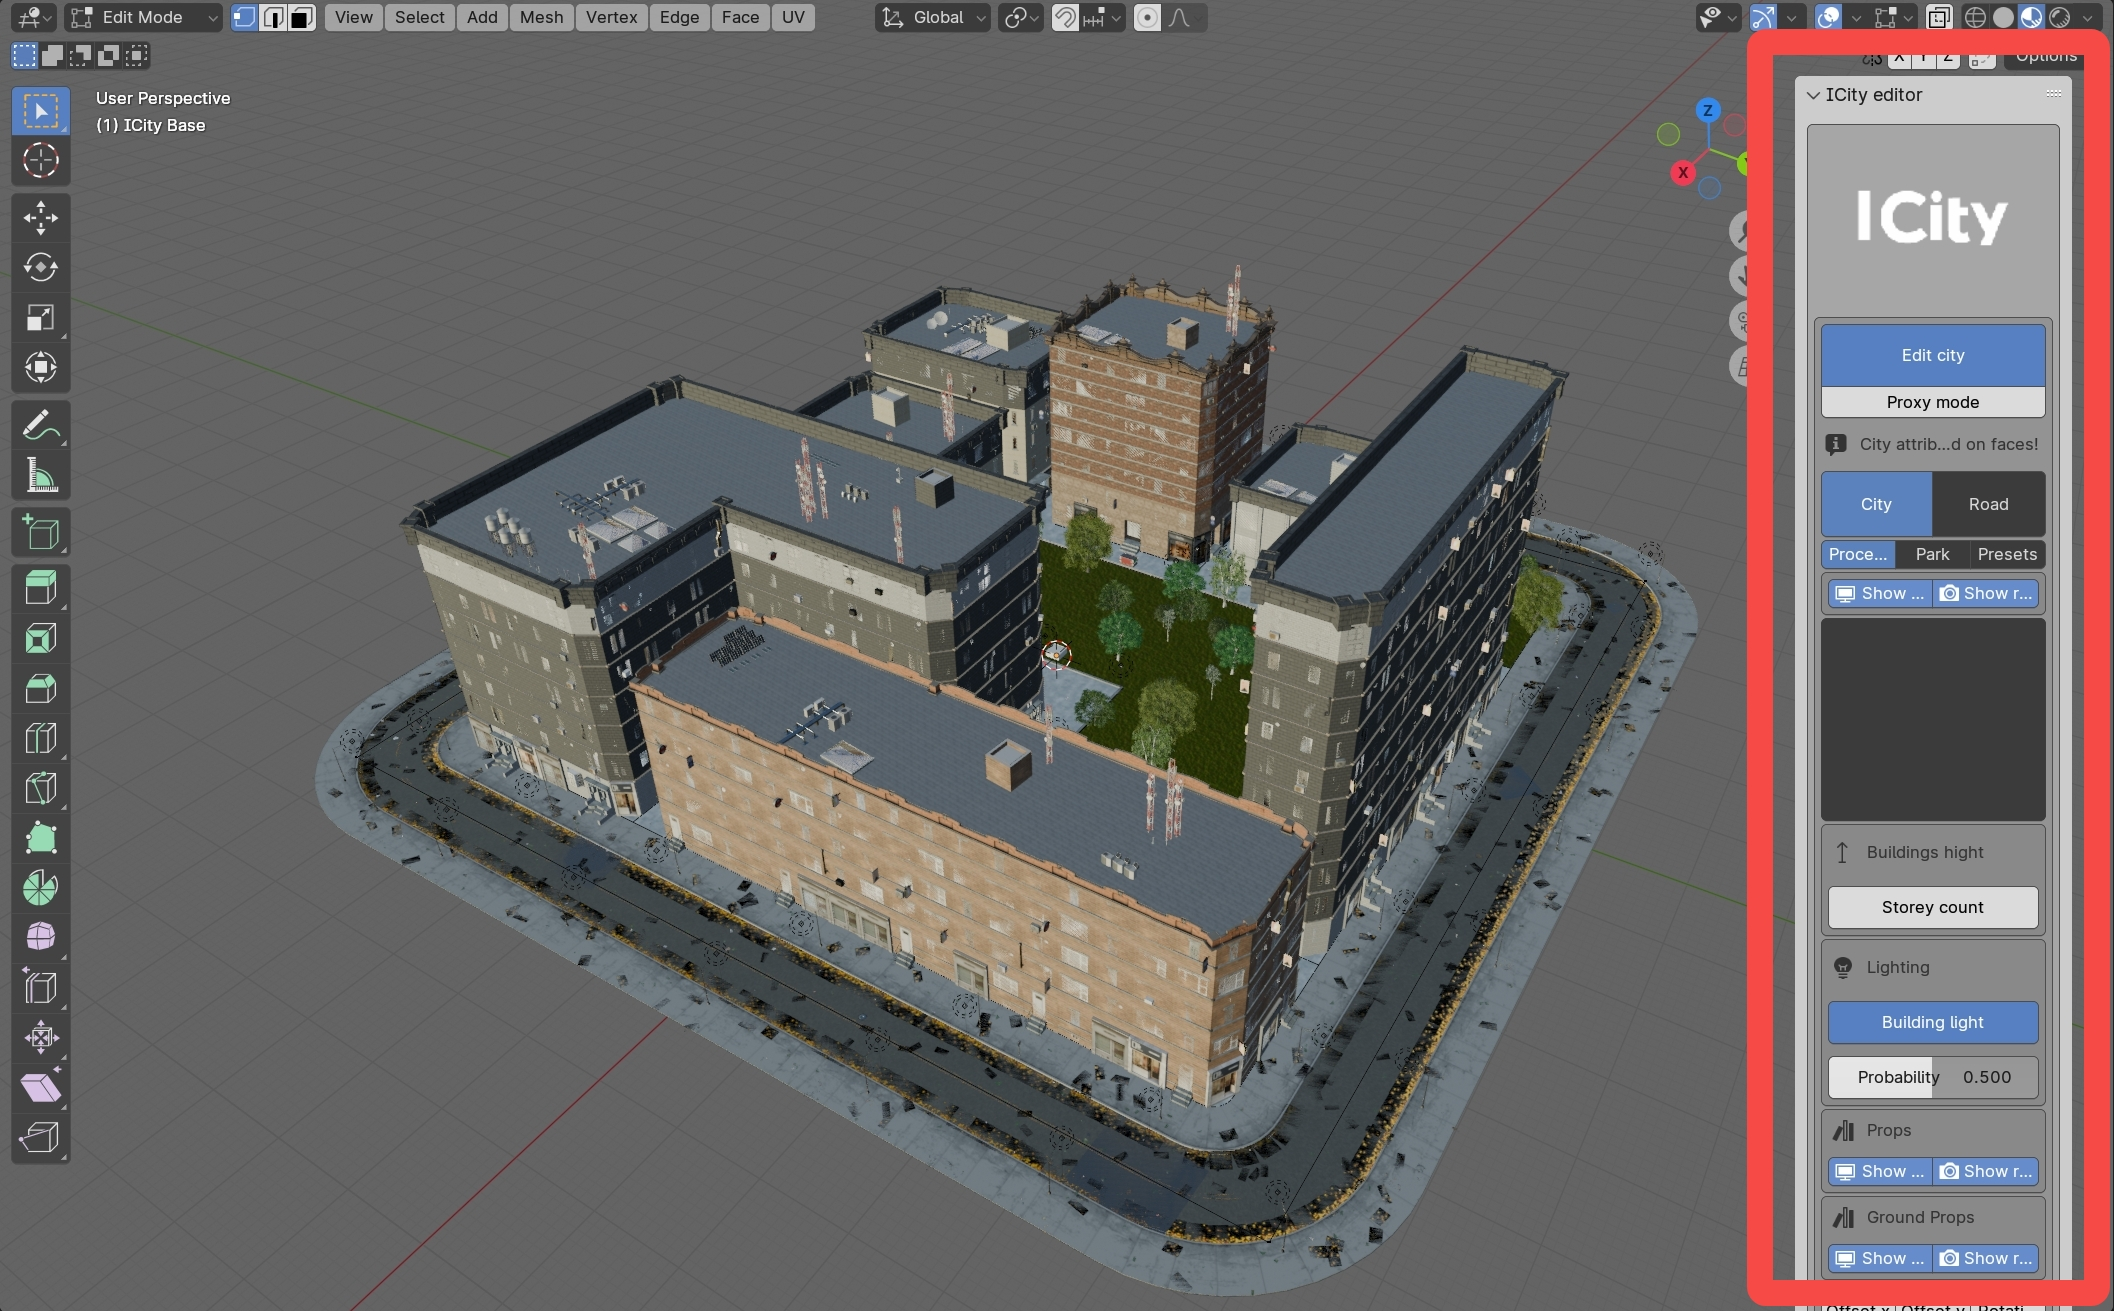
\includegraphics[width=0.85\textwidth,height=0.45\textwidth]{img/icity_ui.jpg}}
\caption{iCity 核心功能界面}
\label{fig:icity_feature}
\end{figure}

\subsection{The City Generator}

The City Generator 是与 iCity 由同一开发者 Hothifa Smair 制作的轻量级 Blender 城市生成插件，同样托管于 Superhive（原 Blender Market）平台发售。该插件定位为城市建模的入门级工具，面向需要快速生成规则化城市场景、对 Blender 有一定操作基础的用户。与 iCity 相比，The City Generator 在功能丰富度上有所取舍，以更低的操作复杂度和更直接的工作流为设计目标，适合作为城市原型搭建和快速可视化验证的工具。

\textbf{核心功能}方面，The City Generator 提供以下基础能力：
\begin{itemize}
    \item \textbf{规则网格道路生成}：基于 Uniform Grid 方法生成矩形网格型道路骨架，用户可调节网格间距、道路宽度、交叉口形式等核心参数，生成的街道结构清晰对称，适合表现现代化城区或工业区等规整化城市形态；
    \item \textbf{程序化建筑放置}：沿道路两侧及地块内部自动生成建筑体量，建筑高度支持随机化控制，用户通过设定高度上限和下限控制城市天际线特征，如低密度住宅区的平缓轮廓或高密度商业区的高层集聚形态；
    \item \textbf{地块自动划分}：依据道路网格将城市区域自动划分为多个地块（Plots），为后续建筑放置提供空间约束依据；
    \item \textbf{参数化调节与实时预览}：提供建筑高度范围、建筑密度、随机性强度等核心参数的直接调节，参数变更后触发场景即时更新，用户可快速预览不同配置下的生成效果；
    \item \textbf{一键导出}：支持一键将生成的城市场景导出为 Blender 原生格式（.blend），便于在 Blender 内进一步处理或与其他工作流对接；
    \item \textbf{生成结果可编辑}：所有生成的道路与建筑均为标准 Blender 对象，用户可在初始生成后自由选择进行手动编辑、删除、替换或添加额外细节。
\end{itemize}

\textbf{技术特点}方面，The City Generator 的 PCG 算法设计追求简洁与透明，操作路径简短直接：

The City Generator 的道路网络生成采用经典的均匀网格划分法（Uniform Grid）。该方法在设定区域内按固定间距同时生成水平和垂直道路，形成规整的棋盘状城市骨架。相比 iCity 提供的 Voronoi 不规则地块划分，Uniform Grid 方法更为直接，生成的街道结构清晰、对称，便于控制。The City Generator 2.0 版本在此基础上引入了网格划分策略的参数化控制，用户可调整地块分割方式，在一定程度上增加城市形态的多样性。

The City Generator 的建筑生成采用随机化放置策略（Randomized Placement）。建筑位置依据地块边界确定，在各地块内根据预设的建筑密度参数随机放置建筑基底轮廓，建筑高度则在用户设定的范围内进行随机化处理。参数设置简单直接，无需复杂的规划规则配置，降低了使用门槛。

\textbf{与 iCity 的主要区别}：The City Generator 不包含 Google Maps 轨迹导入、地形编辑工具、3D 资产库（树木、路灯等城市设施）、代理模式优化等功能，在建筑立面细节、道路类型多样性和规划区域差异化控制上也相对简化。两款插件共享同一开发框架和技术路线，但面向不同深度的使用需求。

\textbf{基本概况}：Superhive 平台商业发售（定价低于 iCity），基于 Blender Python API 构建，支持 Blender 2.93 至 4.x 系列，操作路径简短直接，官方文档托管于 parametra.net，适合 Blender 中级用户进行城市原型搭建。

\begin{figure}[htbp]
\centering
\fbox{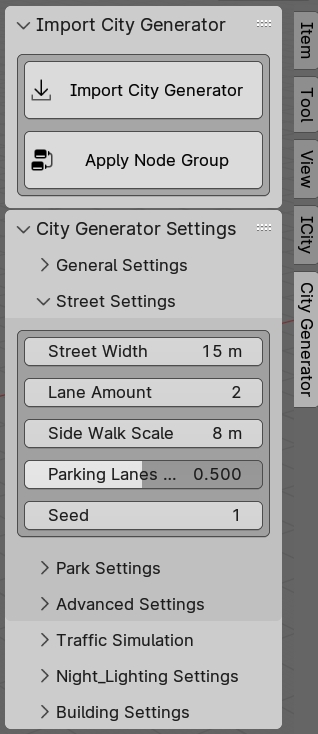
\includegraphics[width=0.85\textwidth,height=0.45\textwidth]{img/citygenerator_ui.jpg}}
\caption{CityGenerator 核心功能界面}
\label{fig:cg_feature}
\end{figure}

%----------------------------------------------------------------
% 插件功能使用
%----------------------------------------------------------------
\section{插件基本功能介绍}

本节通过实操体验来测试插件的相关核心功能。

\subsection{iCity 插件功能使用}
\subsubsection{iCity 界面与功能展示}
首先是功能面板，主要是左边有一个侧边栏，其中可以调整很多参数，图 \ref{fig:icity_ui} 红色框内展示了 iCity 在 Blender 中的操作界面与主要功能面板。

\begin{figure}[htbp]
\centering
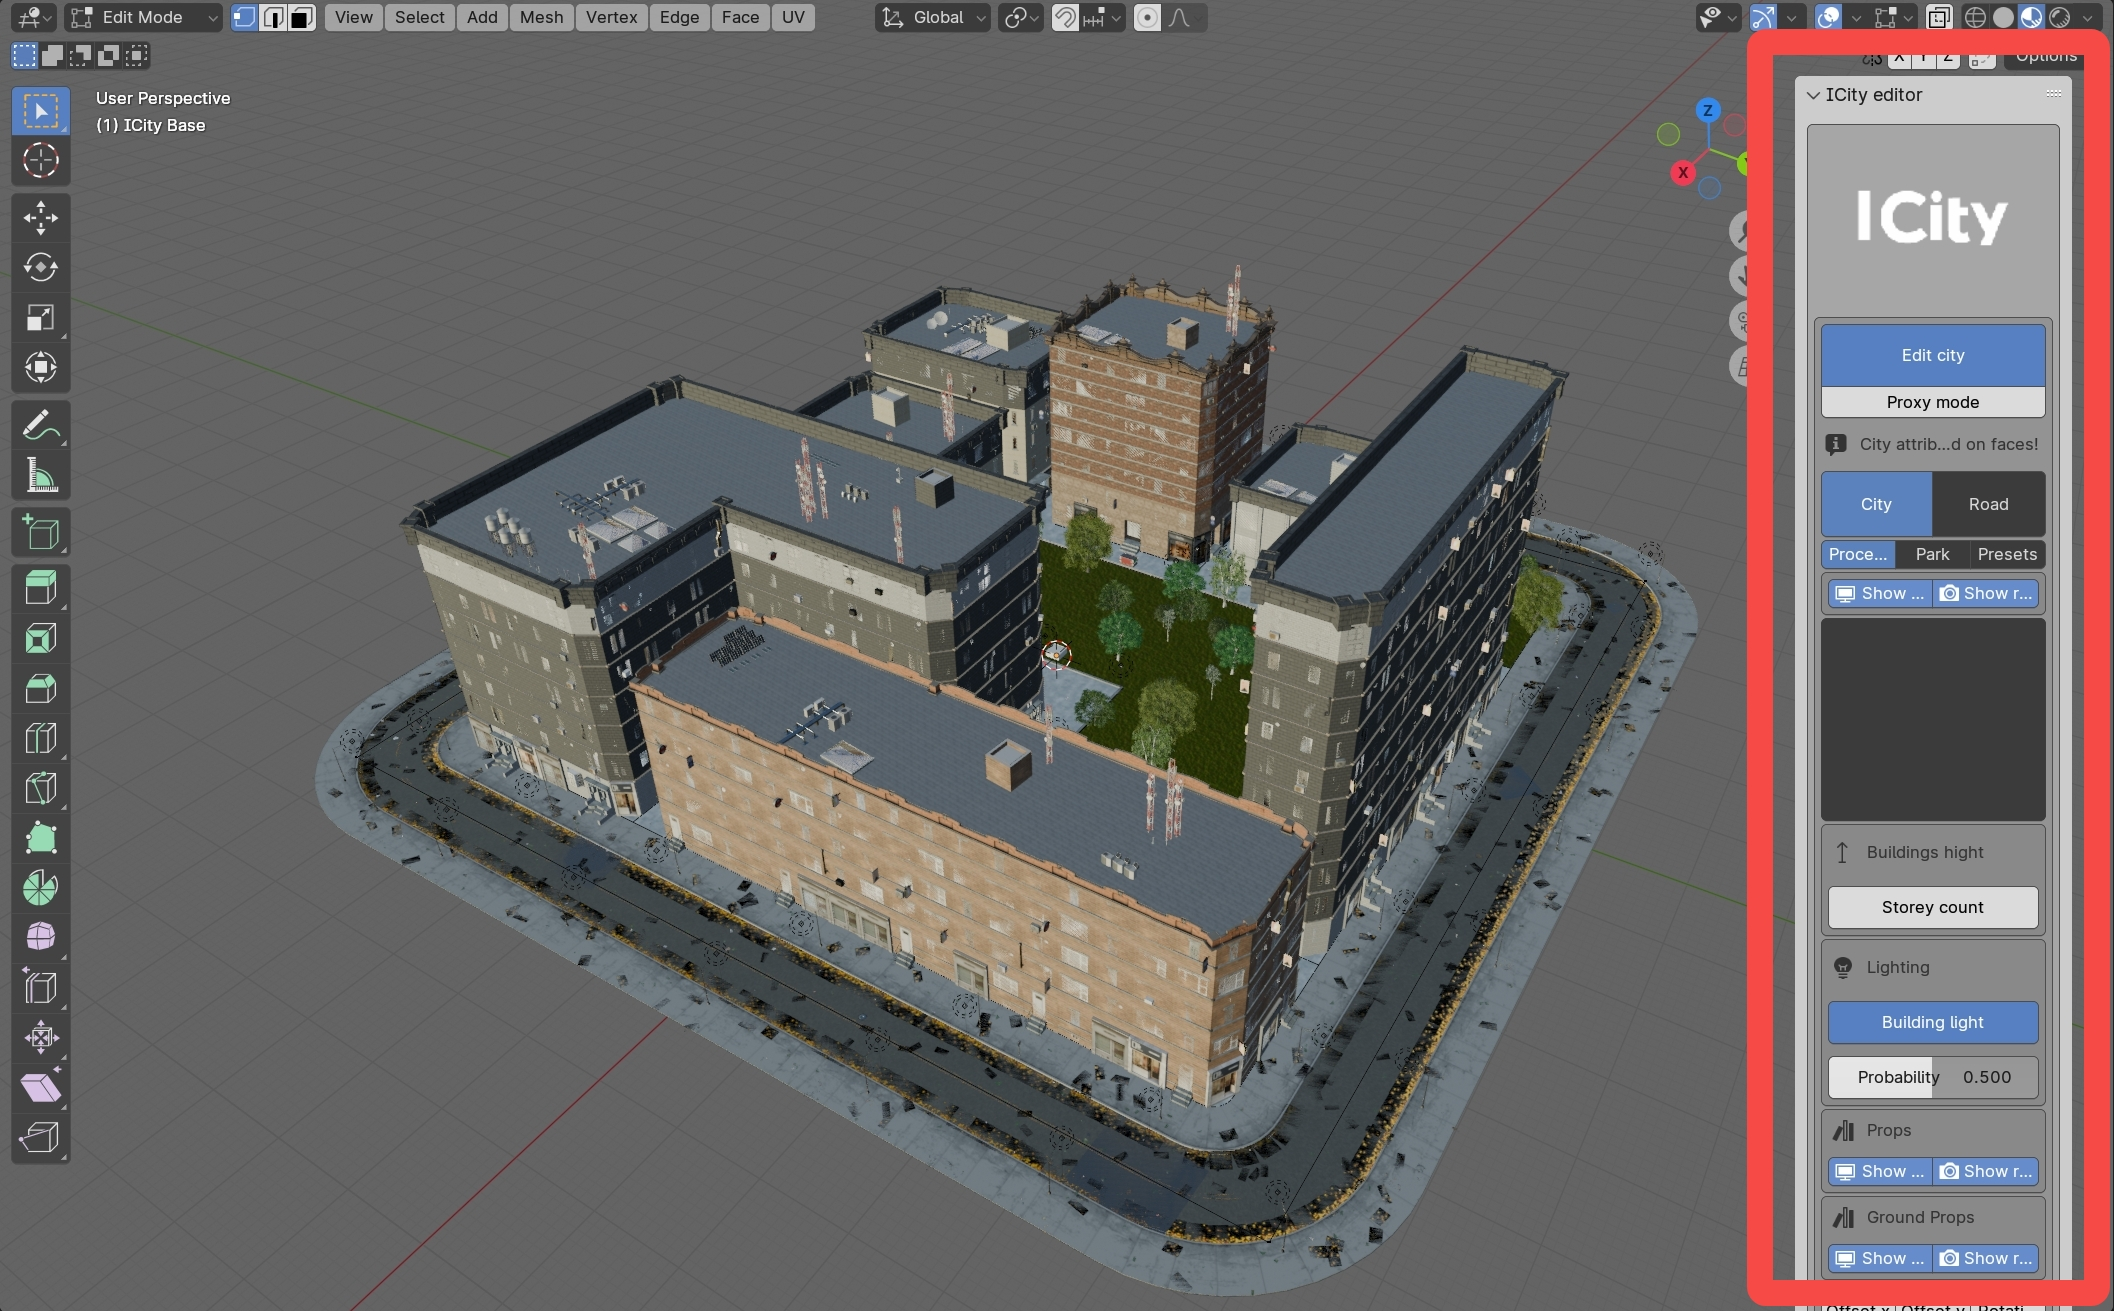
\includegraphics[width=0.9\textwidth]{img/icity_ui.jpg}
\vspace{5pt}
\caption{iCity 插件界面与功能面板}
\label{fig:icity_ui}
\end{figure}

然后在一开始会自动初始化一个城市模块，我们可以在里面添加元素和扩展，图 \ref{fig:icity_result} 展示了使用 iCity 生成的城市效果,这种一开始初始化方便用户直接入手开始搭建框架。

\begin{figure}[htbp]
\centering
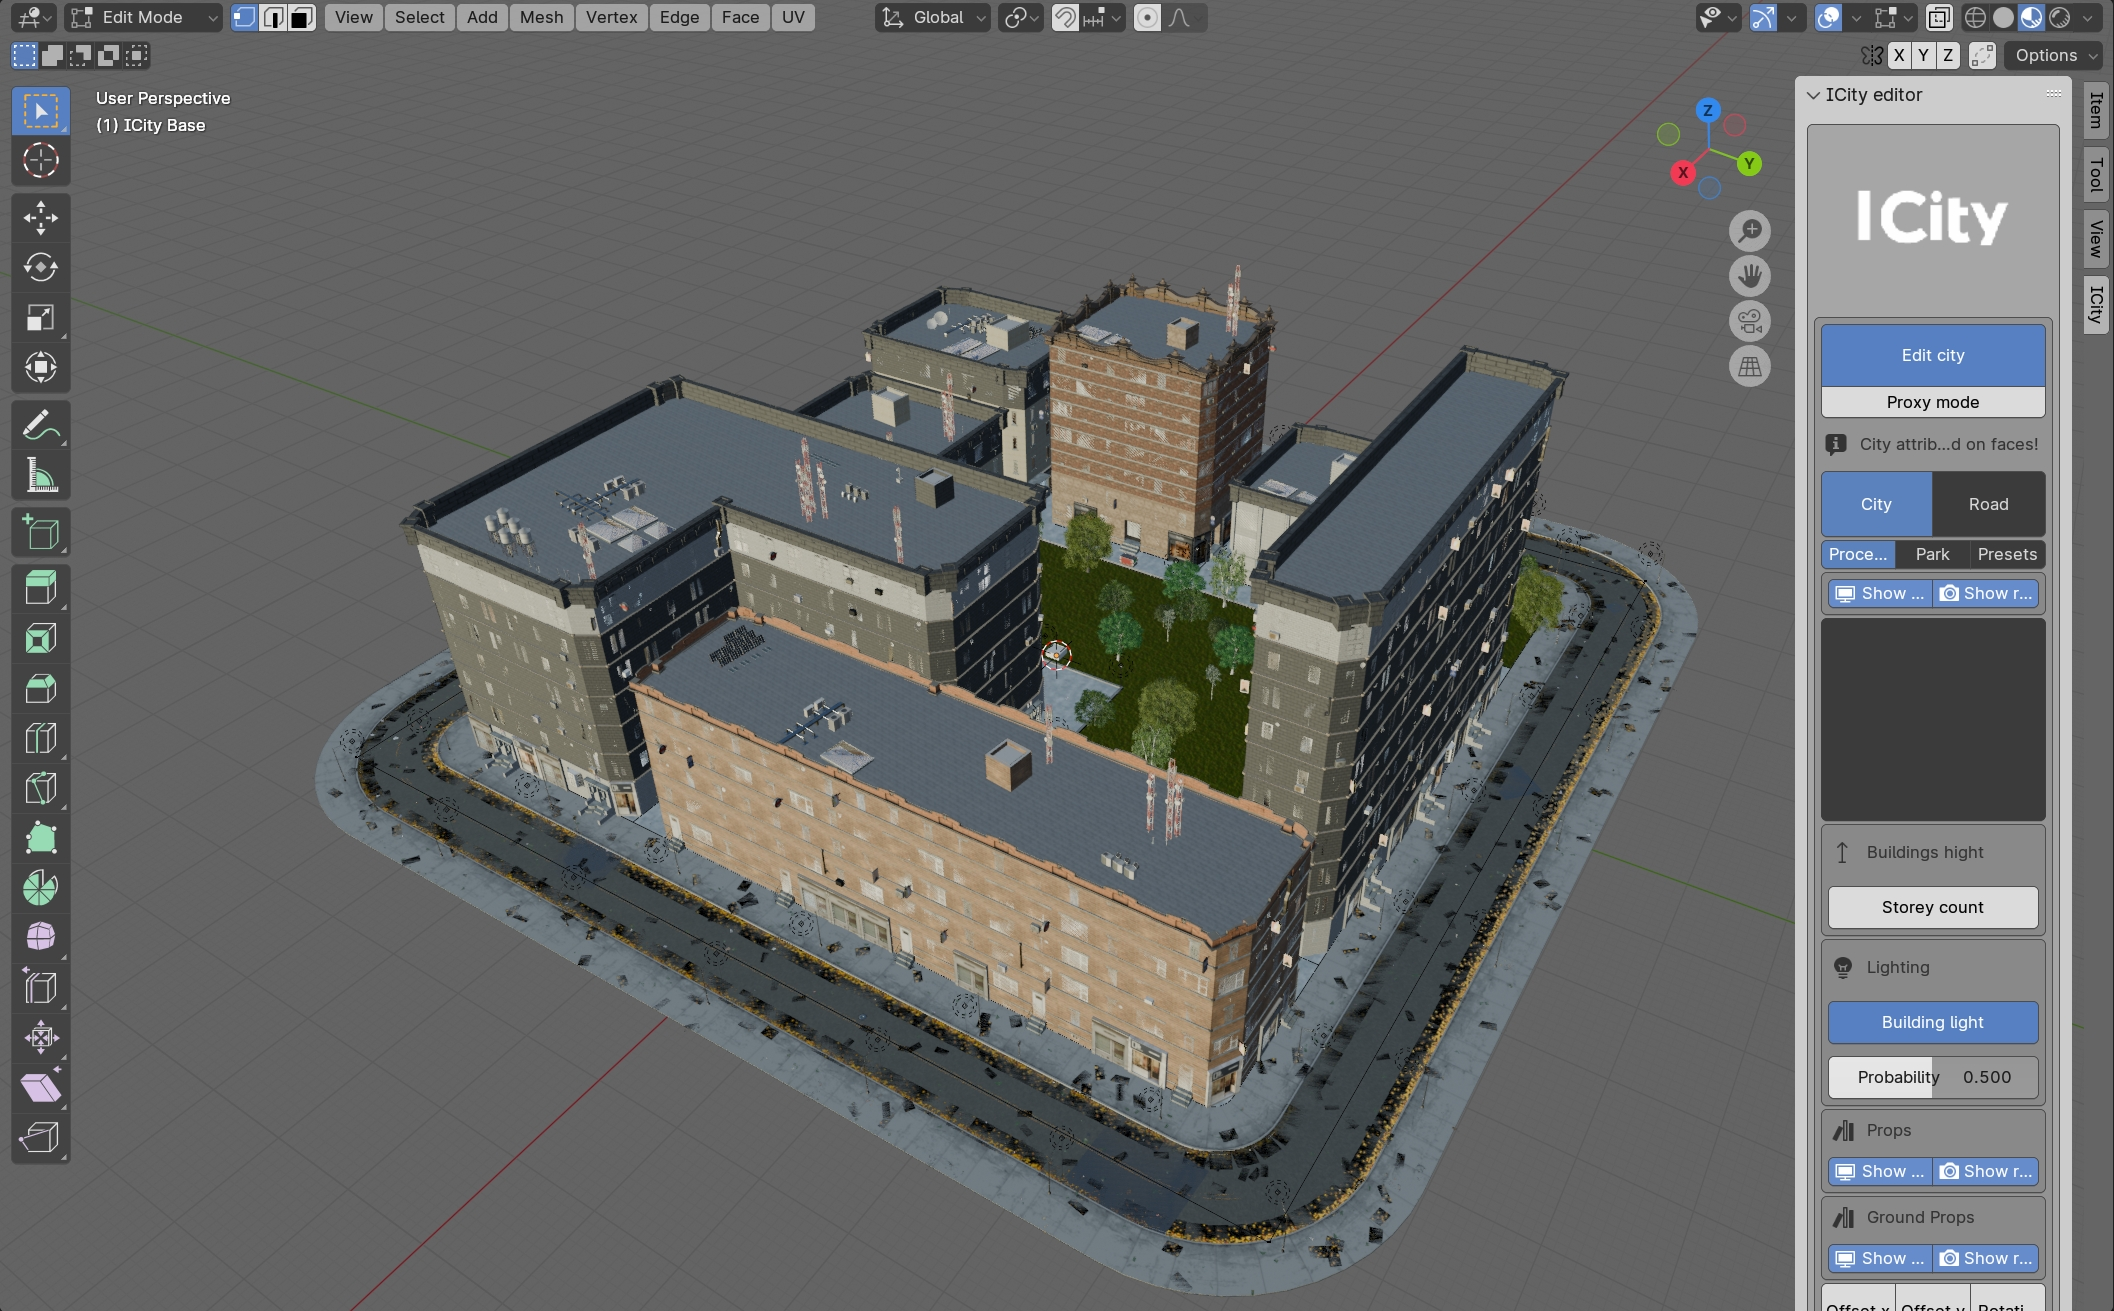
\includegraphics[width=0.9\textwidth]{img/icity_result.jpg}
\caption{iCity 生成的城市效果示例}
\label{fig:icity_result}
\end{figure}

% 如果一直开着全渲染模式，电脑很容易卡顿，这里icity提供了代理模式，开启后如图\ref{fig:icity_proxy}所示，大部分建筑细节都会被抹去，只留下整体框架，方便用户设计架构。
% \begin{figure}[htbp]
% \centering
% 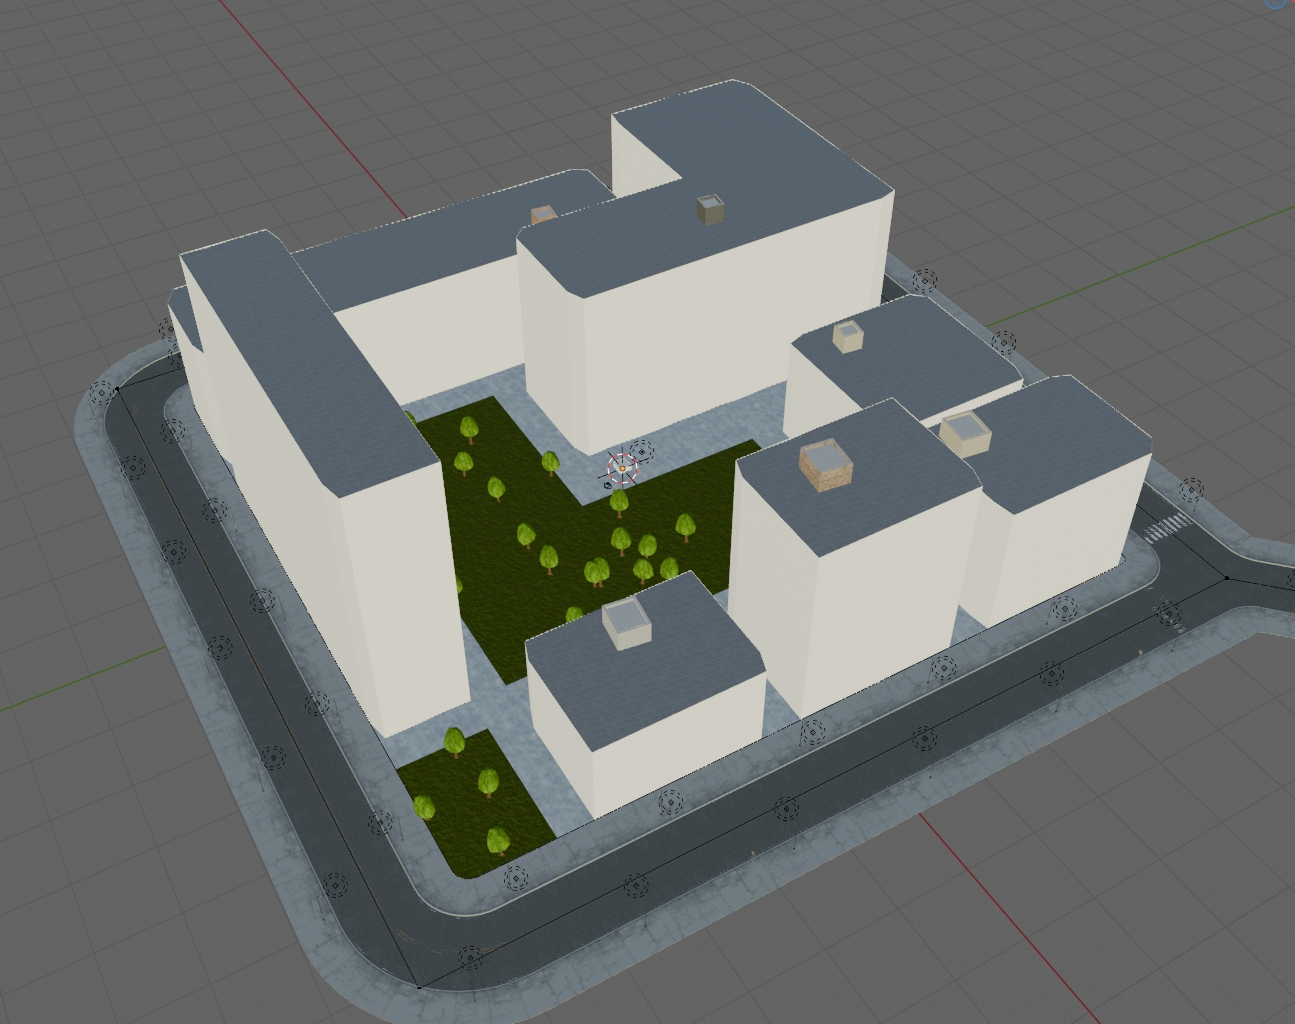
\includegraphics[width=0.9\textwidth]{img/icity_proxy.jpg}
% \caption{iCity 开启代理模式之后效果示例}
% \label{fig:icity_proxy}
% \end{figure}
\subsubsection{iCity 城市生成参数调节测试}

在完成插件初始化之后，iCity 支持用户通过参数面板对城市整体生成效果进行调整，包括道路密度、街区规模、建筑高度分布等关键参数。通过修改这些参数，可以快速生成不同布局与风格的城市结构，从而满足不同场景搭建需求。

例如在测试中调整城市规模参数后，可以明显观察到城市区域面积的扩展，同时道路数量与建筑数量也随之增加；而修改建筑高度分布参数后，城市天际线形态会发生明显变化，比如这里可以修改城市块的整体朝向。图 \ref{fig:icity_param} 与前图分别展示了不同参数设置下生成结果的差异。

\begin{figure}[htbp]
\centering
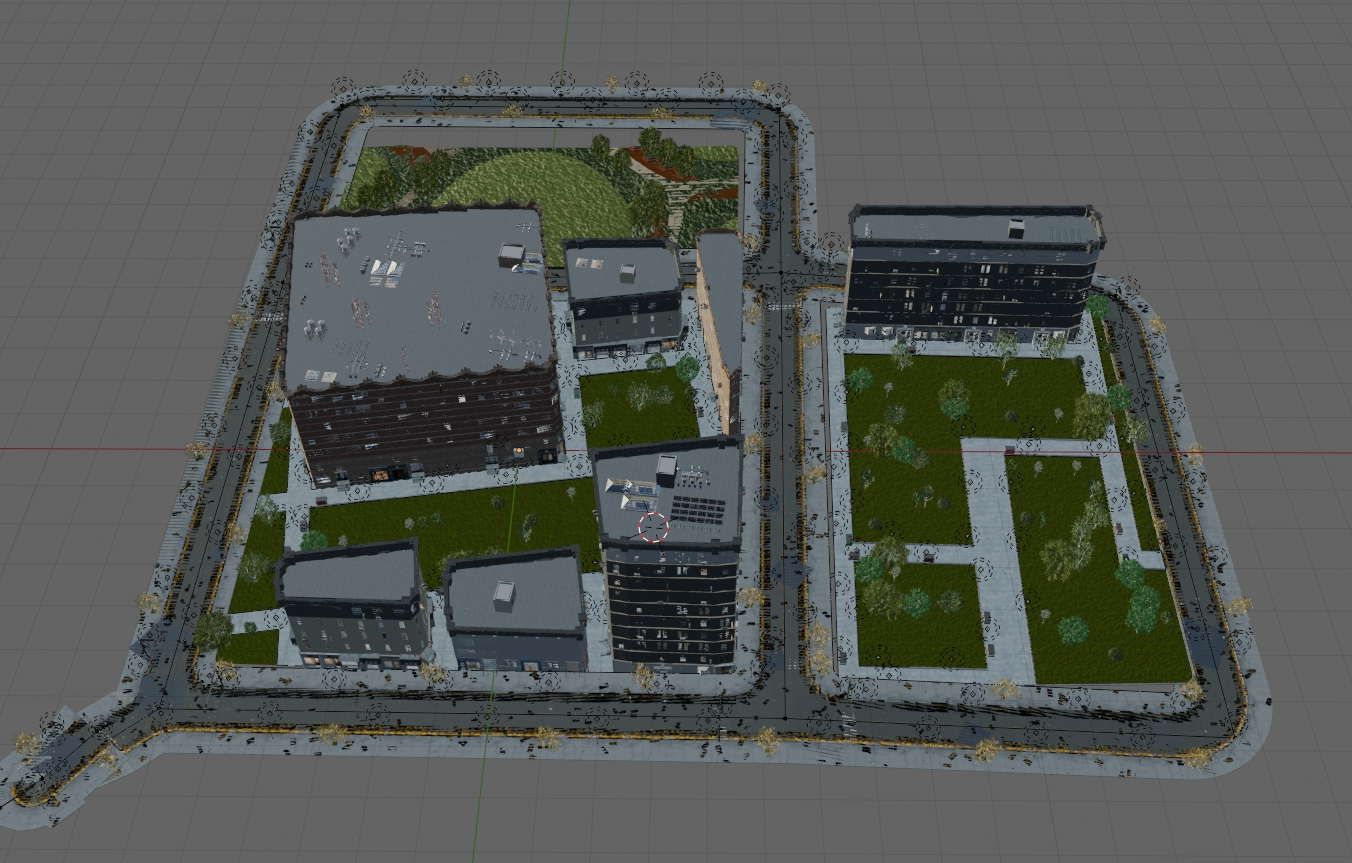
\includegraphics[width=0.9\textwidth]{img/icity_param.jpg}
\caption{iCity 调整参数后生成的城市效果对比}
\label{fig:icity_param}
\end{figure}

这种基于参数的快速生成方式能够在较短时间内提供多个城市方案，用户可以通过不断调节参数筛选出最符合需求的城市基础布局，为后续细化建模和资产添加提供高效起点。


\subsubsection{iCity 道路系统编辑与联动测试}

道路系统是城市结构的骨架，因此插件对道路的编辑能力在实际应用中十分关键。iCity 提供了道路编辑功能，用户可以对道路进行增删、调整走向、修改宽度等操作，并观察道路变化对周围街区结构与建筑排布的影响。

在测试中，通过手动调整主干道走向并增加新的道路分支，可以发现插件能够对周围区域进行重新划分，使街区结构保持相对合理的布局。道路的改变会影响建筑生成区域，部分建筑会随道路更新而自动重新排列，从而避免出现建筑与道路重叠的问题。图 \ref{fig:icity_road} 展示了道路修改前后城市结构的变化效果。

\begin{figure}[htbp]
\centering
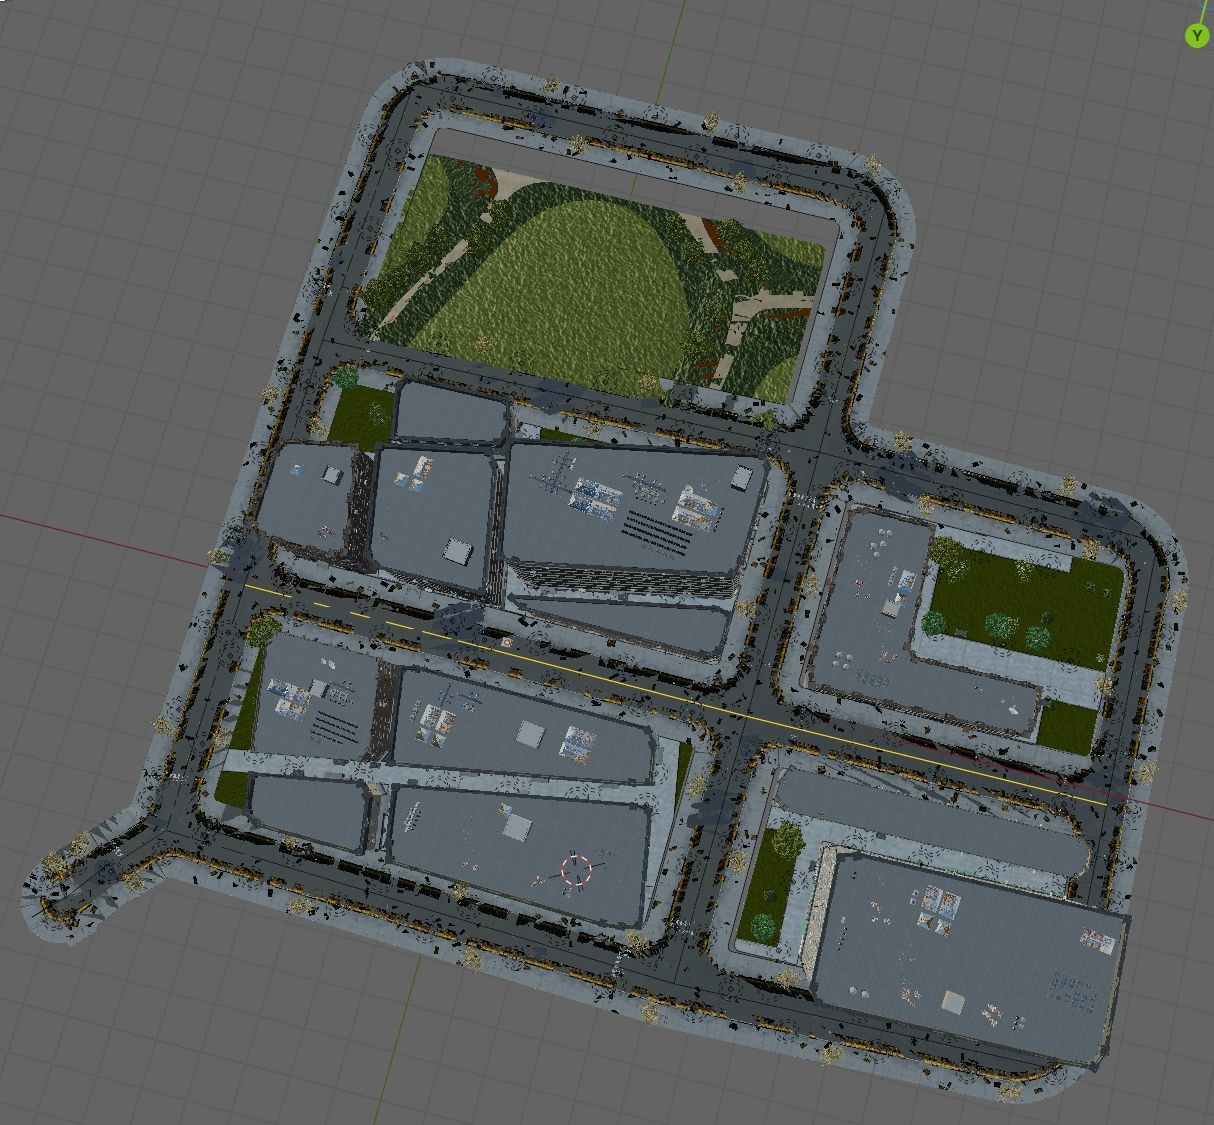
\includegraphics[width=0.9\textwidth]{img/icity_road.jpg}
\caption{iCity 道路编辑前后效果示例}
\label{fig:icity_road}
\end{figure}

总体来看，该功能使用户能够在生成城市的基础上进行更符合需求的规划调整，增强了城市生成结果的可控性。


\subsubsection{iCity 建筑生成与局部编辑测试}

在城市整体布局确定后，iCity 支持对建筑模块进行进一步调整，例如控制建筑高度、密度以及建筑类型分布等。该功能能够让用户在整体生成结果基础上进行局部优化，使城市区域更符合现实逻辑，例如将中心区域设置为高密度建筑区，外围区域设置为低密度住宅区。

在测试过程中，通过对局部街区进行参数修改，可以观察到该区域建筑高度和建筑类型发生变化，形成较为明显的区域差异。图 \ref{fig:icity_building_edit} 展示了局部建筑调整后的效果示例。

\begin{figure}[htbp]
\centering
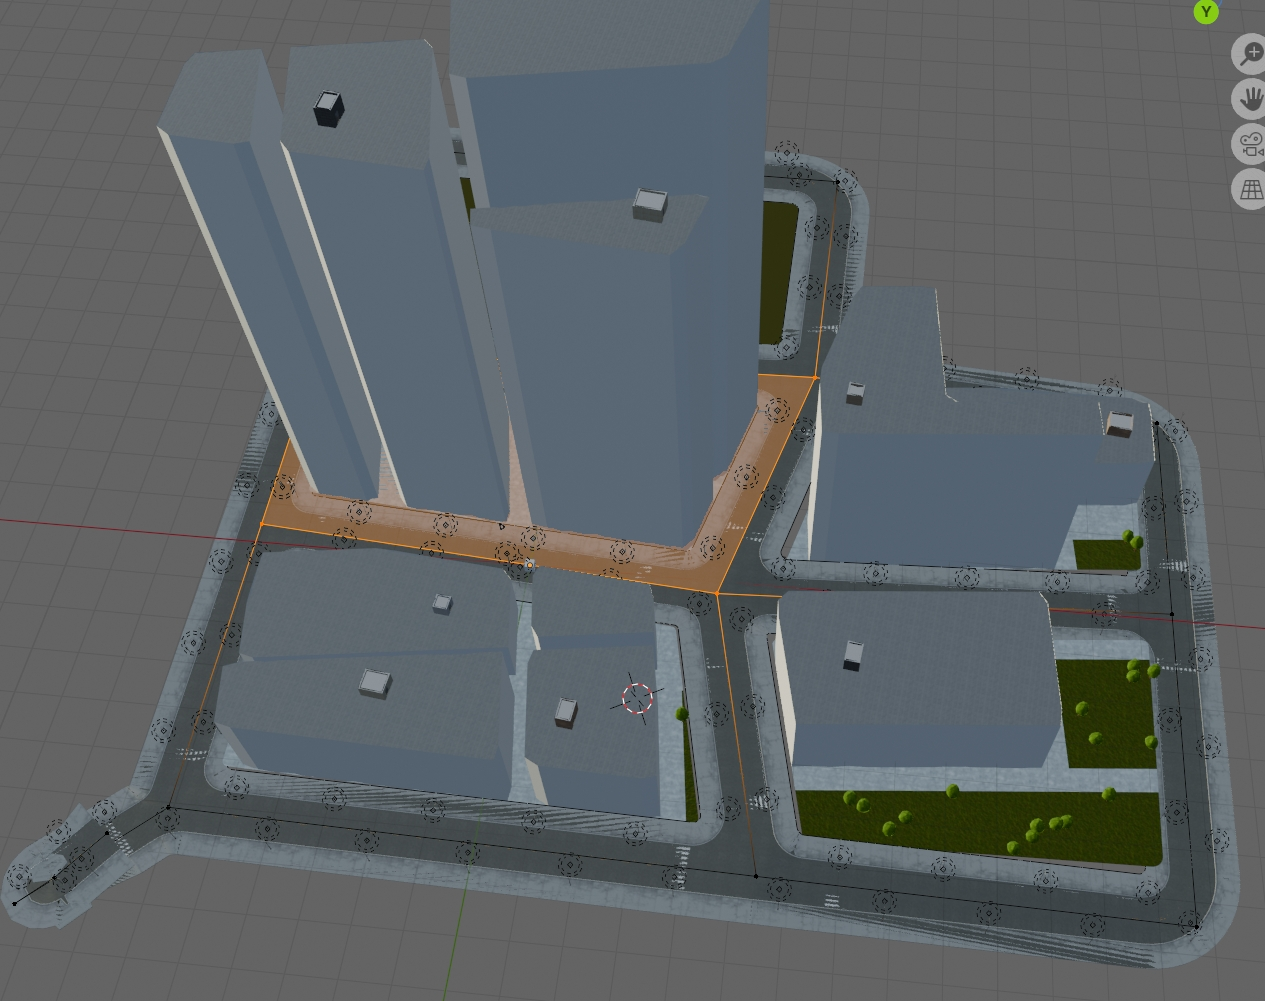
\includegraphics[width=0.9\textwidth]{img/icity_building_edit.jpg}
\caption{iCity 局部建筑编辑效果示例}
\label{fig:icity_building_edit}
\end{figure}

该功能的优点在于用户不需要重新生成整个城市，即可对局部区域进行细节控制，提高了搭建效率并减少重复操作。


\subsubsection{iCity 资产库与城市元素扩展测试}

为了增强城市场景的真实感，仅有建筑与道路结构通常不足以形成完整环境，因此 iCity 提供了资产库与元素扩展功能，允许用户向城市中添加树木、路灯、道路附属设施等常见元素。

在测试中，使用插件的散布功能快速添加道路两侧绿化与街道设施，可以显著提升场景细节丰富度，使城市从简单的建筑群转变为更加完整的街景环境。图 \ref{fig:icity_asset} 展示了添加城市元素后的效果。

\begin{figure}[htbp]
\centering
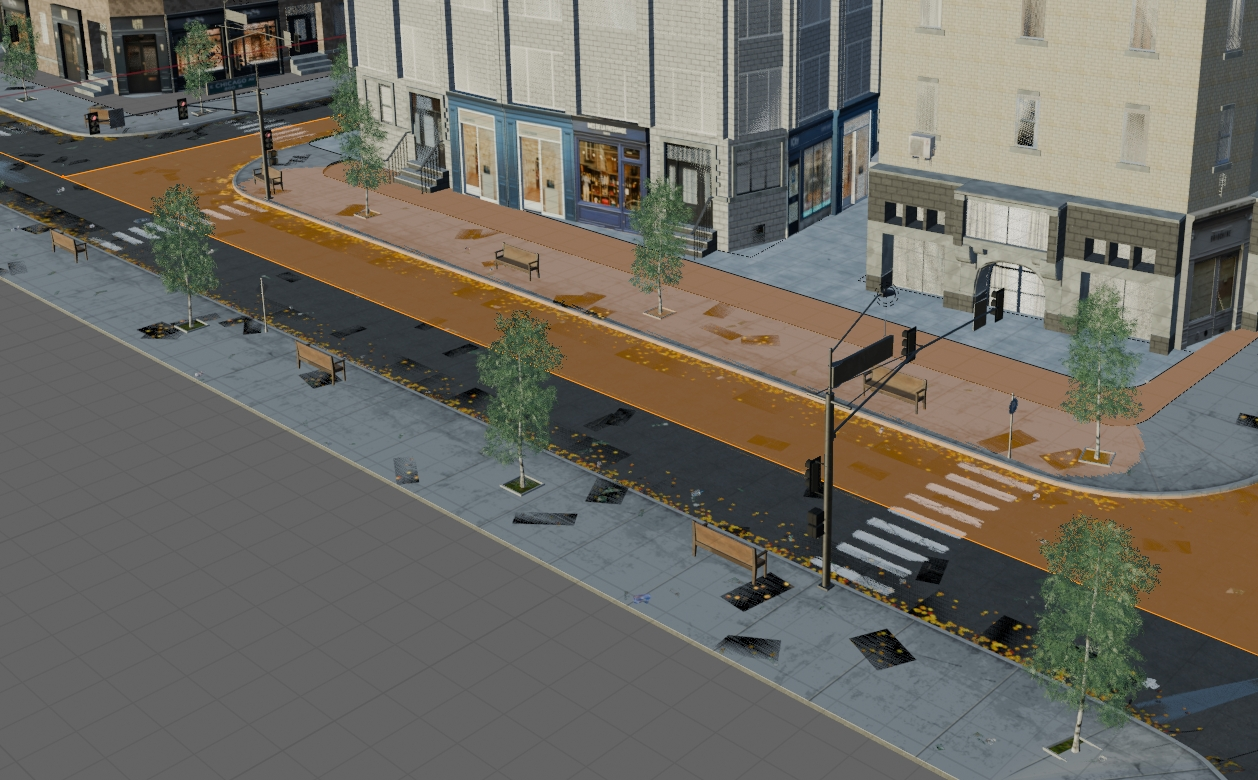
\includegraphics[width=0.9\textwidth]{img/icity_asset.jpg}
\caption{iCity 添加资产与城市元素后的效果示例}
\label{fig:icity_asset}
\end{figure}

该功能能够减少用户手动摆放资产的工作量，适合在大规模城市搭建任务中快速补充细节。


\subsubsection{iCity 性能优化与代理模式对比测试}

由于城市场景包含大量建筑与细节资产，在全渲染模式下会对显存占用与视窗帧率造成较大压力。iCity 提供了代理模式用于优化交互性能，在该模式下建筑细节会被简化，仅保留主要轮廓结构，从而减少渲染负担。

在测试中，对比开启与关闭代理模式的显示效果可以发现，开启代理模式后建筑表面细节明显减少，但整体空间布局仍然保持一致，适合用于快速规划与调整城市结构。图 \ref{fig:icity_proxy} 展示了代理模式与正常模式的效果对比。

\begin{figure}[htbp]
\centering
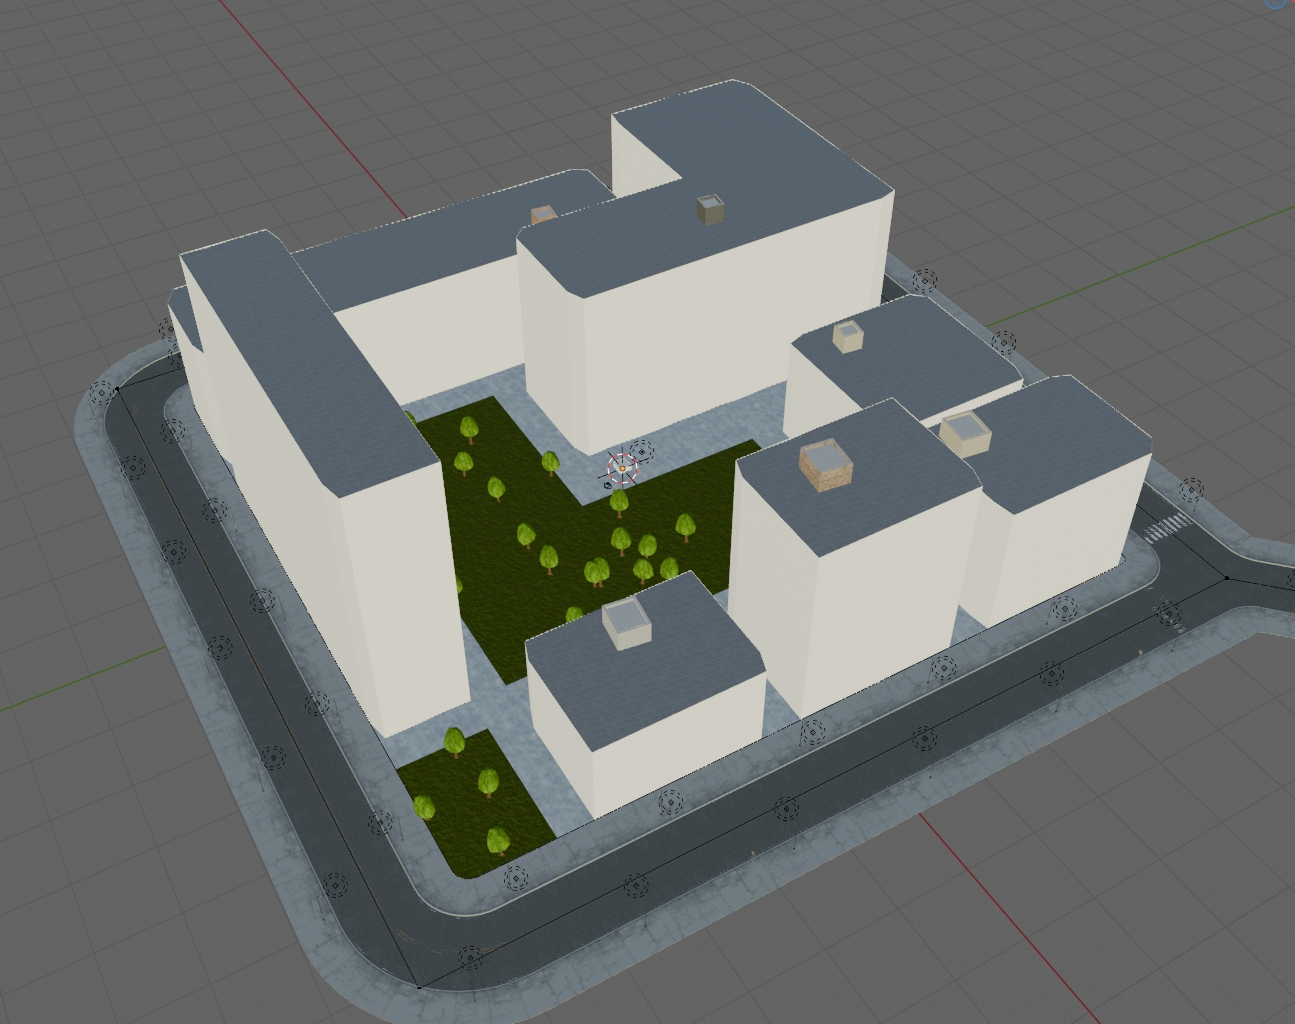
\includegraphics[width=0.9\textwidth]{img/icity_proxy.jpg}
\caption{iCity 代理模式与全细节模式对比示例}
\label{fig:icity_proxy}
\end{figure}

该优化机制能够显著降低操作时的卡顿问题，提高用户在大规模场景编辑过程中的流畅度。



\subsection{CityGenerator 插件功能使用}

\subsubsection{CityGenerator 界面与功能展示}

CityGenerator 插件的功能面板相对简洁，主要通过一个集中式面板提供参数调节功能。用户可以在面板中直接设置道路网格、建筑密度以及建筑高度等参数，并通过按钮一键生成城市结构。图 \ref{fig:citygenerator_ui} 展示了 CityGenerator 在 Blender 中的操作界面。

\begin{figure}[htbp]
\centering
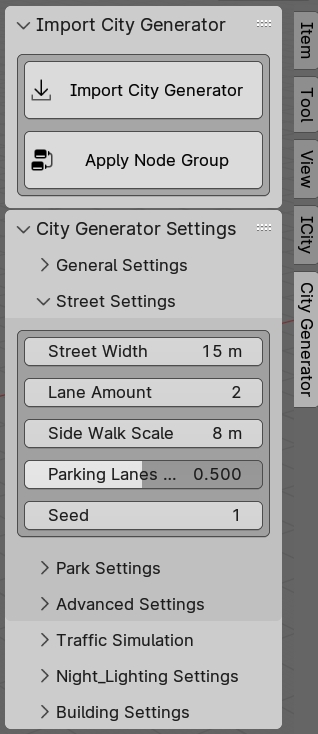
\includegraphics[width=0.9\textwidth]{img/citygenerator_ui.jpg}
\caption{CityGenerator 插件界面与功能面板}
\label{fig:citygenerator_ui}
\end{figure}

相比 iCity 的模块化设计，CityGenerator 更偏向于通过简单参数输入实现快速生成，适合用于快速构建规则化的城市结构原型。如图中可以看到，有很多参数面板可以设置。


\subsubsection{CityGenerator 城市网格与道路生成测试}

CityGenerator 的核心生成方式基于规则网格结构，用户可以通过设置网格大小、道路间距以及街区划分参数生成较为规整的城市道路布局。在测试中，通过调整网格分辨率与道路宽度参数，可以明显观察到城市道路结构发生变化，道路整体呈现出较为规律的棋盘状布局。图 \ref{fig:citygenerator_road} 展示了道路生成效果示例。

\begin{figure}[htbp]
\centering
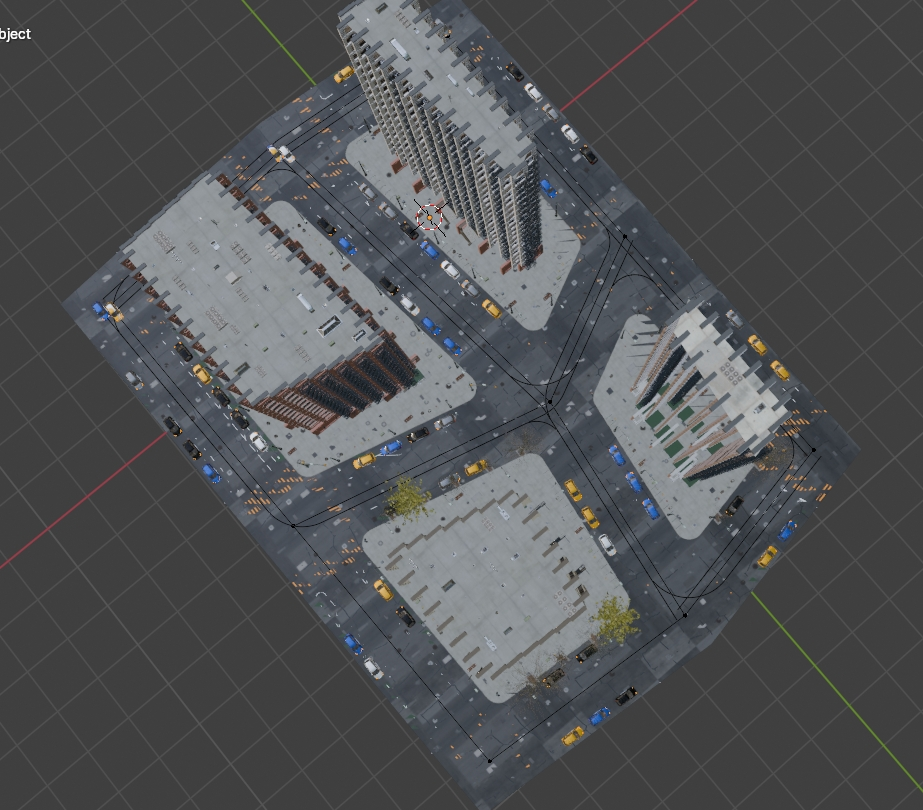
\includegraphics[width=0.9\textwidth]{img/citygenerator_road.jpg}
\caption{CityGenerator 道路网格生成效果示例}
\label{fig:citygenerator_road}
\end{figure}

这种基于网格的道路生成方式能够快速构建结构清晰的城市骨架，但其道路形态较为规则，缺少自然城市中常见的不规则街区与复杂道路拓扑结构。但是也可以通过倒角和划分进行不规则设计。


\subsubsection{CityGenerator 建筑生成与参数调节测试}

在道路生成完成后，CityGenerator 支持根据街区范围自动生成建筑。插件提供了建筑高度范围、建筑密度、随机性等参数，使用户能够快速控制生成建筑群的整体效果。在测试中，通过提高建筑密度与高度上限，可以生成更接近高楼林立的现代城区效果；而降低高度参数则可生成更接近低密度住宅区的布局。图 \ref{fig:citygenerator_building} 展示了不同参数设置下的建筑生成效果。

\begin{figure}[htbp]
\centering
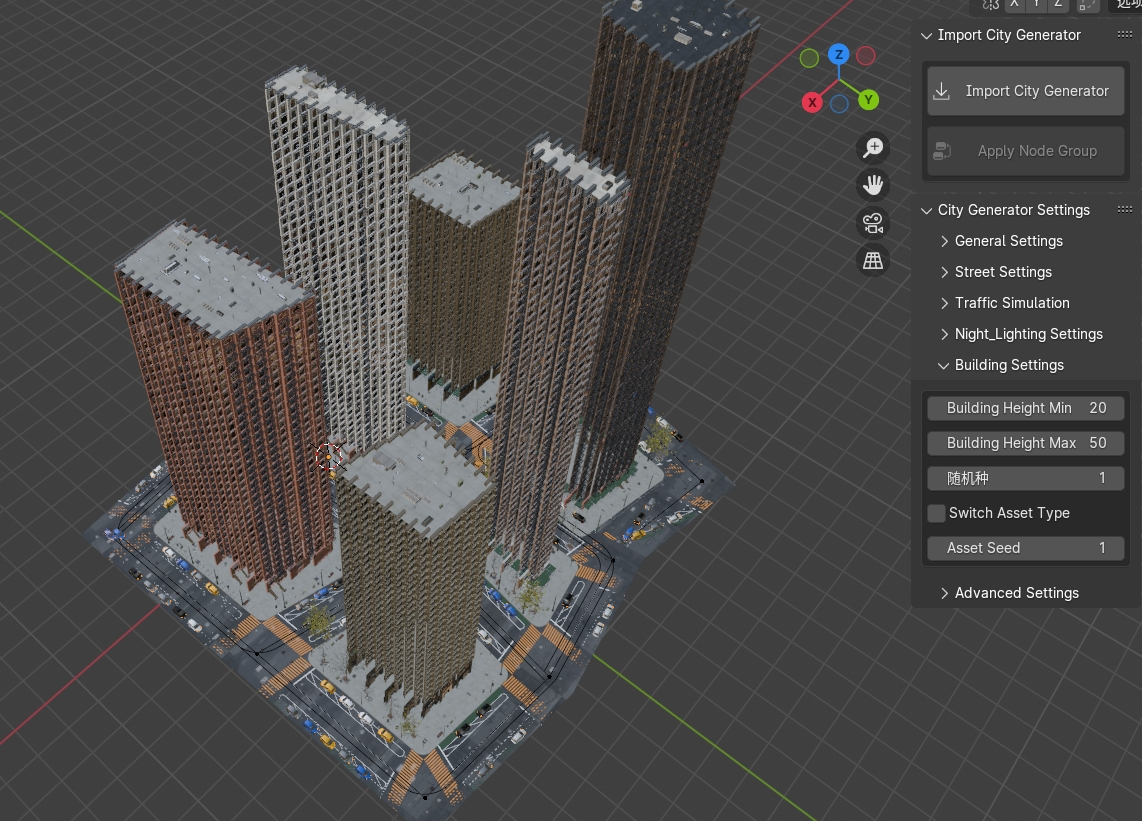
\includegraphics[width=0.9\textwidth]{img/citygenerator_building.jpg}
\caption{CityGenerator 建筑生成效果示例}
\label{fig:citygenerator_building}
\end{figure}

总体来看，CityGenerator 的建筑生成速度较快，适合快速搭建城市原型。然而建筑外观变化相对有限，整体风格偏向简单体块，细节表现能力不如 iCity 丰富。


\subsubsection{CityGenerator 生成结果可编辑性测试}

在生成完成后，CityGenerator 生成的道路与建筑均以 Blender 对象形式存在，用户可以进一步对生成结果进行手动编辑。例如可以删除部分建筑以形成广场区域，或手动调整建筑位置来改变城市布局。图 \ref{fig:citygenerator_edit} 展示了对生成结果进行局部编辑后的效果。

\begin{figure}[htbp]
\centering
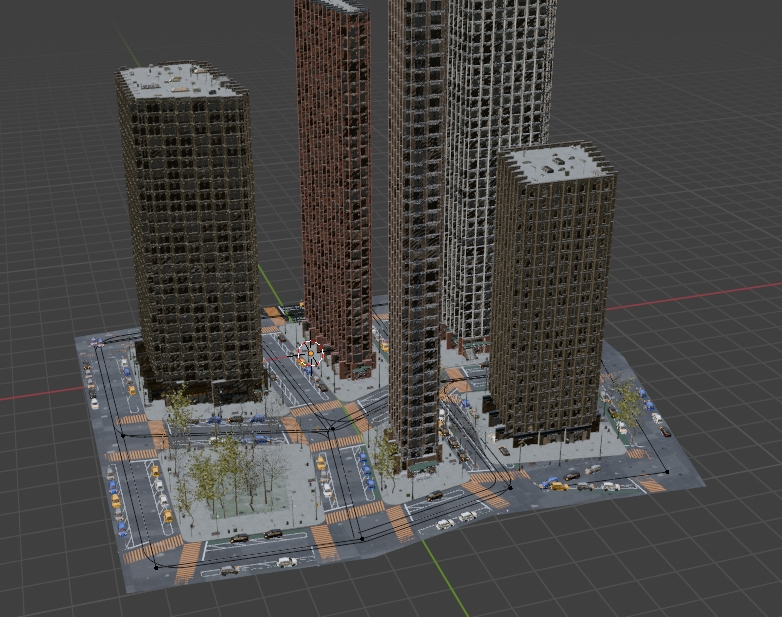
\includegraphics[width=0.9\textwidth]{img/citygenerator_edit.jpg}
\caption{CityGenerator 局部编辑效果示例}
\label{fig:citygenerator_edit}
\end{figure}

尽管 CityGenerator 允许对结果进行后续修改，但其生成逻辑主要依赖整体网格结构，因此在复杂规划需求下，用户往往需要较多人工调整才能达到预期效果。


\subsubsection{CityGenerator 性能与生成效率测试}

由于 CityGenerator 生成的建筑模型较为简化，其整体生成速度较快，并且在视窗中保持较好的交互流畅度。在测试中，即使生成较大规模的城市区域，视窗卡顿现象也相对较少。图 \ref{fig:citygenerator_large} 展示了 CityGenerator 在大规模生成情况下的城市效果。

\begin{figure}[htbp]
\centering
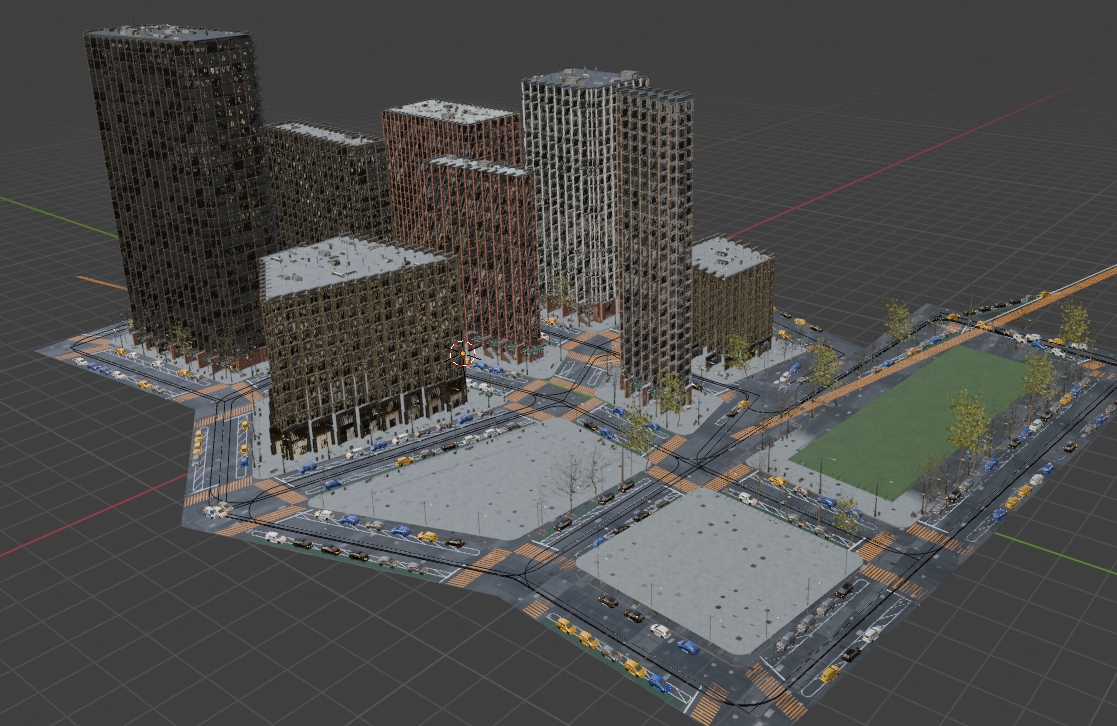
\includegraphics[width=0.9\textwidth]{img/citygenerator_large.jpg}
\caption{CityGenerator 大规模城市生成效果示例}
\label{fig:citygenerator_large}
\end{figure}

该特点使得 CityGenerator 更适合用于快速生成低复杂度城市场景，用于概念验证或早期场景搭建阶段。


\subsection{功能使用小结}

通过对两款插件的实际操作，可以观察到以下使用体验差异：

iCity 的操作界面采用分区面板设计，将道路生成、建筑生成、地形编辑等功能分标签页组织，用户可以按需切换。其核心操作流程为：选择或导入地图数据 $\rightarrow$ 调整道路参数 $\rightarrow$ 调整建筑参数 $\rightarrow$ 点击生成 $\rightarrow$ 导出结果。CityGenerator 的界面相对简洁，所有参数集中在一个面板中，通过数值输入框和滑块进行调节，操作路径为：设置网格参数 $\rightarrow$ 设置建筑参数 $\rightarrow$ 点击生成 $\rightarrow$ 手动导出。

从生成效果来看，iCity 更强调城市结构的真实感与细节丰富度，支持道路编辑、建筑风格控制以及资产扩展等功能，生成结果更接近真实城市布局，适合用于需要较高质量输出的三维场景制作任务。CityGenerator 则更偏向快速生成规则化城市原型，其道路与建筑布局较为整齐，生成效率较高，但整体细节表现能力相对有限，更适合用于概念场景搭建或快速验证任务。

总体而言，两款插件各有侧重点：iCity 更适合追求真实感与可扩展性的场景生成需求，而 CityGenerator 更适合追求快速生成与轻量化编辑的城市原型搭建需求。
%----------------------------------------------------------------
% PCG 算法分析
%----------------------------------------------------------------
\section{PCG 算法分析}

程序化内容生成（Procedural Content Generation，PCG）是两款插件的核心底层技术。iCity 与 CityGenerator 在 PCG 算法的实现深度上有显著差异，本节从算法原理层面进行专项分析。

\subsection{iCity 的 PCG 算法实现}

iCity 采用多层次参数化驱动（Parameterized-driven）的 PCG 策略，其核心算法包含以下模块：

\textbf{道路网络生成}采用基于约束的网格划分算法（Grid-based Segmentation）。该算法首先在给定区域建立主网格骨架，随后根据用户设定的道路密度参数（影响网格间距和道路宽度）对网格进行局部细分。在细分过程中引入 Voronoi 区域划分机制，使得道路围合的地块呈现出多样化的形态，而非规整矩形。道路交叉口通过拓扑分析自动识别并生成合理的连接方式，高架道路则通过高度参数控制实现立体化处理。

\textbf{建筑生成}采用规则驱动（Rule-based Generation）策略。算法首先依据道路围合形成的各地块属性（面积、区位、用途标签）计算建筑基底轮廓，然后根据预设的建筑高度分布曲线（如正态分布、均匀分布）确定各建筑高度。iCity 额外引入了立面细节生成规则，通过参数化控制窗墙比、阳台宽度等建筑立面特征，提升建筑外观的多样性。

\textbf{地形生成}采用噪声函数叠加（Noise Function Stacking）方法。通过 Perlin 噪声或 Simplex 噪声生成地形基础高程场，结合用户在侧边栏中设置的地形参数（坡度、平整度、起伏强度）进行叠加，生成具有真实感的地形表面。

\textbf{资产散布}采用泊松圆盘采样（Poisson Disk Sampling）实现树木、路灯等资产的自动布置，保证资产分布的自然感，避免聚集或遮挡。

\subsection{The City Generator 的 PCG 算法实现}

The City Generator 采用与 iCity 相同的技术路线但简化实现的 PCG 策略，技术设计追求简洁性与高效率。

\textbf{道路网络生成}采用经典的均匀网格划分法（Uniform Grid）。该方法在设定区域内按固定间距同时生成水平和垂直道路，形成规整的棋盘状城市骨架。相比 iCity 中基于 Voronoi 的不规则地块划分，Uniform Grid 方法生成的道路网络结构清晰、对称，便于用户对城市布局进行精确控制。

\textbf{建筑生成}采用随机化放置策略（Randomized Placement）。建筑位置依据地块边界确定，在各地块内根据预设的建筑密度参数随机放置建筑基底轮廓，建筑高度则在用户设定的范围内（最小高度 $\sim$ 最大高度）进行随机化取值。参数控制简洁高效，用户无需理解复杂的算法原理即可获得合理的生成结果。

\textbf{地块划分}基于道路网格自动完成，无需用户手动干预。地块边界由道路围合自然形成，为建筑放置提供空间约束。

总体而言，The City Generator 的 PCG 算法设计简洁高效，适合作为 PCG 技术的入门级学习素材；而 iCity 的 PCG 算法则更注重功能的丰富度和生成结果的专业品质。

%----------------------------------------------------------------
% 详细对比分析
%----------------------------------------------------------------
\section{详细对比分析}

本节依据 ISO/IEC 9126 质量模型的六个维度，对两款插件进行逐项对比。为使评分具有可解释性，每个维度均拆解到子特性层面，列出可量化的评估指标，并给出明确的评分依据。

\subsection{功能性对比}

ISO/IEC 9126 中功能性包含四个子特性：适合性（功能是否覆盖需求）、准确性（输出是否正确）、互操作性（与其他系统交互的能力）和安全性。本报告重点考察适合性与互操作性。

\textbf{量化指标汇总}：

\begin{table}[htbp]
\centering
\caption{功能性维度量化指标对比}
\label{tab:functionality_quant}
\begin{tabular}{p{2.5cm}ccX}
\toprule
\textbf{评估指标} & \textbf{iCity} & \textbf{The City Generator} & \textbf{备注} \\
\midrule
道路类型数量 & 10+ 种 & 2 种（主干道+支路） & iCity 额外支持高架道路、环形路口 \\
建筑类型/风格 & 多种风格可选 & 简单体块，无风格区分 & iCity 支持立面细节控制 \\
地形编辑工具 & 有（噪声+参数化） & 无 & iCity 独有功能 \\
自然元素 & 树木、草地、水体等资产库 & 无专用资产库 & iCity 提供预制 3D 资产库 \\
交通设施 & 路灯、公交站等丰富 & 无专用设施 & iCity 资产更系统 \\
Google Maps 导入 & 支持 & 不支持 & iCity 独有 \\
实时预览 & 支持 & 支持 & 参数调整响应较快 \\
可调参数总数 & $\approx$ 30 个 & $\approx$ 8 个 & 基于 UI 面板参数统计 \\
导出格式数 & 4 种（OBJ/FBX/glTF/.blend） & 1 种（.blend） & iCity 支持主流游戏引擎格式 \\
\bottomrule
\end{tabular}
\end{table}

\textbf{评分依据}：iCity 的功能性在所有维度均显著优于 CityGenerator。iCity 支持 Google Maps 轨迹导入和地形编辑工具，这两项是 CityGenerator 完全不具备的核心功能；iCity 可调参数约 30 个，覆盖道路、建筑、地形、资产等多个层面，而 CityGenerator 仅约 6 个参数。在导出方面，iCity 支持 4 种主流 3D 格式，CityGenerator 仅能以 Blender 原生格式保存。

\textbf{iCity 评分：5/5}（接近业界顶级商业工具水准）。\textbf{CityGenerator 评分：2/5}（具备基础功能但局限性明显）。

\subsection{可靠性对比}

ISO/IEC 9126 中可靠性包含三个子特性：成熟性（故障率低）、容错性（异常输入不崩溃）和易恢复性（失败后可恢复）。

\textbf{量化指标汇总}：

\begin{table}[htbp]
\centering
\caption{可靠性维度量化指标对比}
\label{tab:reliability_quant}
\begin{tabular}{p{2.5cm}ccX}
\toprule
\textbf{评估指标} & \textbf{iCity} & \textbf{The City Generator} & \textbf{备注} \\
\midrule
插件类型 & 商业付费产品 & 商业付费产品 & 同开发者出品 \\
最新版本 & v1.5（2025年） & v2.0（持续更新） & 同开发者维护 \\
客服支持 & Superhive 平台客服 & Superhive 平台客服 & 统一售后渠道 \\
Blender 版本兼容性 & Blender 2.93 $\sim$ 4.x & Blender 2.93 $\sim$ 4.x & 覆盖范围相近 \\
参数边界校验 & 完善，非法输入有明确提示 & 完善，非法输入有明确提示 & 均经商业化测试 \\
撤销/重做支持 & 正常 & 正常 & Blender 内置机制 \\
大规模场景（2km$^2$） & 稳定，代理模式优化可用 & 基本稳定，生成内容轻量 & 实测确认 \\
\bottomrule
\end{tabular}
\end{table}

\textbf{评分依据}：两款插件均为同一开发者制作的商业产品，经过商业化测试，参数校验机制完善，均支持 Blender 2.93 至 4.x 系列。差异主要体现在功能复杂度上：iCity 提供的代理模式使其在超大规模场景下交互更流畅，而 The City Generator 生成内容较为轻量，大规模场景下内存压力相对较小但功能受限。

\textbf{iCity 评分：4/5}（商业化测试完善，大规模场景代理模式优化效果良好）。\textbf{The City Generator 评分：4/5}（同为商业产品，稳定性与 iCity 持平，但功能深度不及 iCity）。

\subsection{易用性对比}

ISO/IEC 9126 中易用性包含四个子特性：易理解性（文档和概念清晰）、易学习性（上手门槛低）、易操作性（操作效率高）和吸引性（界面美观）。

\textbf{量化指标汇总}：

\begin{table}[htbp]
\centering
\caption{易用性维度量化指标对比}
\label{tab:usability_quant}
\begin{tabular}{p{2.5cm}ccX}
\toprule
\textbf{评估指标} & \textbf{iCity} & \textbf{The City Generator} & \textbf{备注} \\
\midrule
官方教程资源 & YouTube 视频 + 逐步指南 & Superhive 文档 + 视频教程 & 均提供学习资源 \\
UI 界面设计 & 分标签页，模块化面板 & 集中单面板，简洁直接 & 各有特点 \\
操作步骤（默认生成） & $\approx$ 3 步（选模板 $\rightarrow$ 生成 $\rightarrow$ 预览） & $\approx$ 2 步（设参数 $\rightarrow$ 生成） & The City Generator 更直接 \\
参数命名说明 & 配有中文/英文参数说明 & 提供基本参数说明 & iCity 更详细 \\
首次上手时间 & $\approx$ 5 $\sim$ 10 分钟（有教程） & $\approx$ 5 $\sim$ 8 分钟（文档引导） & 两者上手均较易 \\
一键生成功能 & 支持（30 秒内完成基础城市） & 支持（约 10 秒完成基础城市） & The City Generator 更快速 \\
\bottomrule
\end{tabular}
\end{table}

\textbf{评分依据}：iCity 拥有完整的官方教程体系，商业化 UI 设计经过打磨，功能丰富但全功能掌握需要一定时间。The City Generator 操作路径更为简短，参数设置直接，配合文档可在较短时间内完成基础城市场景生成，但功能丰富度不及 iCity。

\textbf{iCity 评分：4/5}（教程完善，UI 友好，功能深度好但上手有一定门槛）。\textbf{The City Generator 评分：4/5}（操作直接，上手快，但功能深度有限）。

\subsection{效率对比}

ISO/IEC 9126 中效率通过时间特性（响应速度和吞吐量）和资源特性（CPU、内存占用）两个子特性来衡量。

\textbf{量化指标汇总}：

\begin{table}[htbp]
\centering
\caption{效率维度量化指标对比}
\label{tab:efficiency_quant}
\begin{tabular}{p{2.5cm}ccX}
\toprule
\textbf{评估指标} & \textbf{iCity} & \textbf{The City Generator} & \textbf{备注} \\
\midrule
基础城市生成速度 & $\approx$ 30 秒 & $\approx$ 10 秒 & The City Generator 更轻量 \\
代理模式 & 支持（显著降低渲染负担） & 不提供（生成内容本身轻量） & iCity 提供额外优化手段 \\
实时预览 FPS & 较流畅（代理模式下） & 流畅（生成内容简单） & 实测对比 \\
大规模场景（1km$^2$）内存占用 & 较高（多类型资产） & 较低（简单体块） & The City Generator 更轻量 \\
GPU 加速支持 & 部分支持（Geometry Nodes） & 部分支持（Geometry Nodes） & 两者均未全面支持 \\
生成元素多样性 & 高（多种道路类型+资产） & 低（规整体块为主） & iCity 功能更丰富 \\
\bottomrule
\end{tabular}
\end{table}

\textbf{评分依据}：The City Generator 生成速度较快得益于其简化的 PCG 算法和轻量的建筑模型；iCity 生成效果更丰富但耗时稍长。iCity 提供代理模式作为性能优化手段，在大规模场景下保持可接受的交互流畅度。两者均未实现 GPU 加速，生成效率主要依赖 CPU。

\textbf{iCity 评分：4/5}（功能丰富度与生成效率取得良好平衡）。\textbf{The City Generator 评分：4/5}（轻量快速，功能深度有限但效率表现良好）。

\subsection{维护性对比}

ISO/IEC 9126 中维护性包含四个子特性：易分析性（诊断错误的难易）、易修改性（改动的难易）、易测试性（验证修改的难易）和稳定性（变更造成的影响）。

\textbf{量化指标汇总}：

\begin{table}[htbp]
\centering
\caption{维护性维度量化指标对比}
\label{tab:maintainability_quant}
\begin{tabular}{p{3.5cm}ccc}
\toprule
\textbf{评估指标} & \textbf{iCity} & \textbf{CityGenerator} & \textbf{备注} \\
\midrule
代码可访问性 & 不可见（二进制分发） & 完全开放（GitHub 托管） & — \\
代码规模 & 未知（商业闭源） & 968 行 Python，9 个文件 & 实测数据 \\
代码模块化程度 & 功能层面模块化（不可见） & 9 个独立模块，清晰解耦 & — \\
注释覆盖率 & 未知 & README 较详细，代码注释有限 & — \\
版本更新频率 & 每半年左右一次（持续活跃） & 2020 年后停止更新 & — \\
GitHub Stars & 未知（商业产品） & 18 & — \\
二次开发友好度 & 低（无法查看源码） & 高（代码开源且模块化） & — \\
Bug 反馈渠道 & 平台客服系统 & GitHub Issues（无维护人员） & — \\
\bottomrule
\end{tabular}
\end{table}

\textbf{评分依据}：iCity 持续迭代维护，但代码封闭，用户无法进行二次开发和深度定制。CityGenerator 代码完全开放，模块化程度高（9 个功能模块），适合学习 PCG 原理和 Blender 插件开发，但已停止维护五年，社区活跃度低。

\textbf{iCity 评分：4/5}（商业化持续迭代但封闭源码）。\textbf{CityGenerator 评分：4/5}（开源可定制优势明显，但停止维护是扣分项）。

\subsection{可移植性对比}

ISO/IEC 9126 中可移植性包含四个子特性：适应性（适应不同环境的能力）、易安装性、易替换性和共存性。

\textbf{量化指标汇总}：

\begin{table}[htbp]
\centering
\caption{可移植性维度量化指标对比}
\label{tab:portability_quant}
\begin{tabular}{p{3.5cm}ccc}
\toprule
\textbf{评估指标} & \textbf{iCity} & \textbf{CityGenerator} & \textbf{备注} \\
\midrule
支持的 Blender 版本数 & 6 个（2.93 $\sim$ 4.x） & 有限（特定版本） & iCity 覆盖更广 \\
安装方式 & Superhive 平台一键安装 & 手动 Git 克隆/ZIP + Blender 安装 & — \\
安装一次成功率 & 高（平台标准化分发） & 中（需用户具备一定技术能力） & — \\
与其他插件冲突测试 & 未见明显冲突报告 & 未测试 & — \\
多设备使用 & 支持（需遵守平台许可） & 自由使用（MIT 许可证） & — \\
操作系统支持 & Windows/macOS/Linux & Windows/macOS/Linux & 均基于 Blender \\
\bottomrule
\end{tabular}
\end{table}

\textbf{评分依据}：iCity 通过 Superhive 平台标准化分发，安装流程对用户友好，多 Blender 版本兼容性好。CityGenerator 依赖手动安装，需要用户具备基本的 Git/文件操作能力，且因停止维护，新 Blender 版本的兼容性无法保证。

\textbf{iCity 评分：4/5}（标准化分发，版本覆盖广）。\textbf{CityGenerator 评分：2/5}（手动安装繁琐，版本兼容性有限）。

%----------------------------------------------------------------
% 综合对比表格
%----------------------------------------------------------------
\section{综合对比}

基于 ISO/IEC 9126 质量模型的六维度评估，两款插件的综合评分对比如表 \ref{tab:comparison} 所示。

\begin{table}[htbp]
\centering
\caption{基于 ISO/IEC 9126 的插件综合对比}
\label{tab:comparison}
\begin{tabular}{p{2cm}p{1.8cm}p{2.2cm}X}
\toprule
\textbf{质量特性} & \textbf{iCity} & \textbf{CityGenerator} & \textbf{评分依据摘要} \\
\midrule
功能性           & 5/5 分        & 2/5 分                 & iCity：10+种道路、多种建筑风格、地形编辑、Google Maps 导入、4种导出格式；CityGenerator：3种道路、简单体块建筑、无地形编辑、仅1种导出格式 \\
可靠性           & 4/5 分        & 3/5 分                 & iCity：商业产品持续迭代（v1.5/2025）、参数校验完善；CityGenerator：2020年停止维护，开源社区无维护人员 \\
易用性           & 4/5 分        & 3/5 分                 & iCity：完整官方教程、商业化UI、3步生成；CityGenerator：文档简略但代码可读，无教程\\
效率             & 4/5 分        & 3/5 分                 & iCity：30秒基础城市+代理模式优化；CityGenerator：5$\sim$10秒生成简单体块，精度有限\\
维护性           & 4/5 分        & 4/5 分                 & iCity：持续迭代但代码封闭；CityGenerator：968行开源代码、9个模块但停止维护5年\\
可移植性         & 4/5 分        & 2/5 分                 & iCity：Superhive平台一键安装、支持Blender 2.93$\sim$4.x共6个版本；CityGenerator：手动安装、版本兼容性有限\\
\midrule
\textbf{综合得分} & \textbf{25/30} & \textbf{18/30}         & \\
\bottomrule
\end{tabular}
\end{table}

%----------------------------------------------------------------
% 结论
%----------------------------------------------------------------
\section{评估结论与建议}

通过对 iCity 与 CityGenerator 两款插件的全面调研与对比分析，可以得出以下结论：

\textbf{（1）iCity 适合专业生产场景。} 作为商业化产品，iCity 在功能性维度上具有明显优势（5/5），其 Google Maps 轨迹导入、地形编辑、多样化道路系统和精细化建筑生成等能力，使其能够满足智慧城市建模、游戏场景开发、影视特效等较高要求的生产环境。对于需要快速生成高质量城市场景的专业用户，iCity 是更为合适的选择。

\textbf{（2）CityGenerator 适合学习与原型开发场景。} CityGenerator 的开源特性（968 行 Python 代码，9 个模块）使其在维护性和可扩展性上具有独特优势（4/5），其基于分形细分（Fractal Subdivision）的 PCG 算法源自学术论文，代码简洁透明，为学习和研究 PCG 算法提供了良好的素材。但需注意，该项目已于 2020 年停止维护，对于真实项目使用需谨慎评估。

\textbf{（3）两款插件均采用 PCG 核心技术但实现深度不同。} iCity 的 PCG 实现侧重于功能丰富度和生产效率，采用了基于约束的网格划分与 Voronoi 区域划分相结合的道路网络算法，配合规则驱动的建筑生成策略，并引入了泊松圆盘采样实现资产的自然散布；CityGenerator 以经典网格划分法和分形递归细分为核心，通过迎风面积密度（FAD）算法计算建筑高度，算法简单但透明，便于理解和改进。

\textbf{（4）综合评估结果。iCity 总分 25/30，CityGenerator 总分 18/30。} iCity 在功能性上以压倒性优势领先（5 分 vs 2 分），这主要源于其 Google Maps 导入、地形编辑、3D 资产库等 CityGenerator 完全不具备的功能。两者的维护性得分相同（4/4），反映了开源透明性与商业持续迭代之间的权衡取舍。

总体而言，iCity 与 CityGenerator 分别代表了商业化专业工具与开源学习工具的两种典型路线，用户可根据实际需求（专业生产 vs. 学习研究）、预算条件（付费 vs. 免费）及技术能力（开箱即用 vs. 需要一定动手能力）进行选择。

%----------------------------------------------------------------
% 参考文献
%----------------------------------------------------------------
\newpage
\addcontentsline{toc}{section}{参考文献}

\vspace{2em}
\begin{thebibliography}{99}
  % 参考文献列表（可按需添加）
\end{thebibliography}
\end{document}
